\documentclass[12pt]{article}
\usepackage{amsmath, amssymb, amsthm, setspace, mathptmx, apalike, graphicx}
%multirow
\usepackage[a4paper, margin=2.5cm]{geometry}

\title{The Relationship of Age, Gender, and Region on Income in Italy}
\author{Enzo Lopes Baitello}


% Bisogno, Matteo (A.A. 2022/2023) Povertà monetaria dal 2004 al 2020: stima probit su microdati dell'indagine sui bilanci delle famiglie italiane condotta dalla Banca d'Italia.
% POLACCHI, BREEZY (2023)Piani Individuali Pensionistici (PIP) e polizze vita: un’analisi econometrica sulle SHIW 2016-2020 di Banca d’Italia.
% Previati, D.A., Ricci, O., Stentella Lopes, F. (2020). La capacità delle famiglie italiane di assorbire lo shock pandemico: il ruolo dell’alfabetizzazione finanziaria. In M. Paoloni (a cura di), L'Italia ai tempi del Covid-19. Vol. 2. Wolters Kluwer Italia srl.
%aaa

\begin{document}

\maketitle

\clearpage
\tableofcontents

\clearpage
\section{Introduction}

\begin{spacing}{1.5}

Trying to understand the effects that age, gender, and region have on Italian income, may help us understand better how the Italian economy works. For a long time Italy has been one of the countries with the greatest rate of unemployment among Europe, this is only one of the different ways on how age affects a persons ability to earn an income. Moreover, by looking a gender, it will be important to first better understand the gender pay gap and what are its causes and if this situation is improving. Also, Italy is well known for the North-South divide of its economy, we will first try to understand from where this stems from and how this has affected the income of people living in the south. Finally, we will try to model all of this issues through econometrics by using a multiple linear regression on data of the Survey on Household Income and Wealth conducted by  the Banca d'Italia.

\end{spacing}

\section[Descriptive Analysis]{Descriptive Analysis \footnote{All of the data mentioned in this section comes from the Istat, \textit{Rilevazione sulle forze di lavoro} if not otherwise stated.}} 

\subsection{Age}

\begin{spacing}{1.5}

Income is strongly affected by a person's ability to get work and stay employed. This is relevant because people who are either very young or very old tend to have difficulties with this. The unemployment for people aged 15-24 in 2022 was 23.7\% while the unemployment rate for people aged 15-74 was 8.1\%. Over time the unemployment rate for the younger age group has gone down substantially over time by 4.3\% since 2010 while the unemployment rate for the 15-74 age group has gone down only by 0.4\%. The age group that saw the greatest increase in the unemployment rate was the 50-74 age group with an increase of 1.2\% from 2010 to 2022. Moreover, we can also see a difference the hourly wage earnings for employees in the private sector between different age groups. The hourly wage for employees in the private sector in the 15-29 age group was €10.42 while the hourly earnings were €13.5 for the 50 or greater age group. The differnce between the two has gone down over time because the hourly earnings for the younger group has increased at a faster rate than that of the older group, the younger group saw an increase of 6.44\% from 2021 and the older age group saw an increase of 1.73\%. 

The unemployment rate for the 25-34 age group was 11.4\%. This age group may be more representative of the young people that are looking for jobs because most of the 15-24 are studying and they represent a very low amount of the unemployed \cite{pontecorvo2018giovani}. This can be seen in the higher non participation rates among the 15-24 age group compared to the 25-34 age group. The non participation rate of the former age group in 2020 was 47.2\% and for the latter it was 25.3\%. There has been a steady increase in the non participation rate among both age groups but it has remained relatively similar for both. Moreover, in times of crisis unemployment among the 15-24 and 25-34 age groups is greater than the average \cite{pontecorvo2018giovani}. Another problem that affects younger age groups more than the older ones is the underemployment rate. For the 15-24 and 25-34 age groups the underemployment rates in 2020 were 6.3\% and 4.8\% respectively while the underemployment rate for the 15-74 age group was 3.7\%. This is because the Italian economy has a relatively low demand for qualified workers and the ones that are needed are probably already employed by older age groups \cite{pontecorvo2018giovani}. Furthermore, there is a greater impact in times of crisis for younger age groups because most of the time they are working short term contracts or part time. The rate of part time workers for the 15-34 age group was 22.7\% in 2020 and 18.88\% for the 35-64 age group. Also, the rate of full time workers decreased for the younger age group decreased by 4.83 points while it increased by 3.93 for the older age group.

\begin{figure}
	\begin{minipage}[b]{0.5\textwidth}
		\begin{center}
			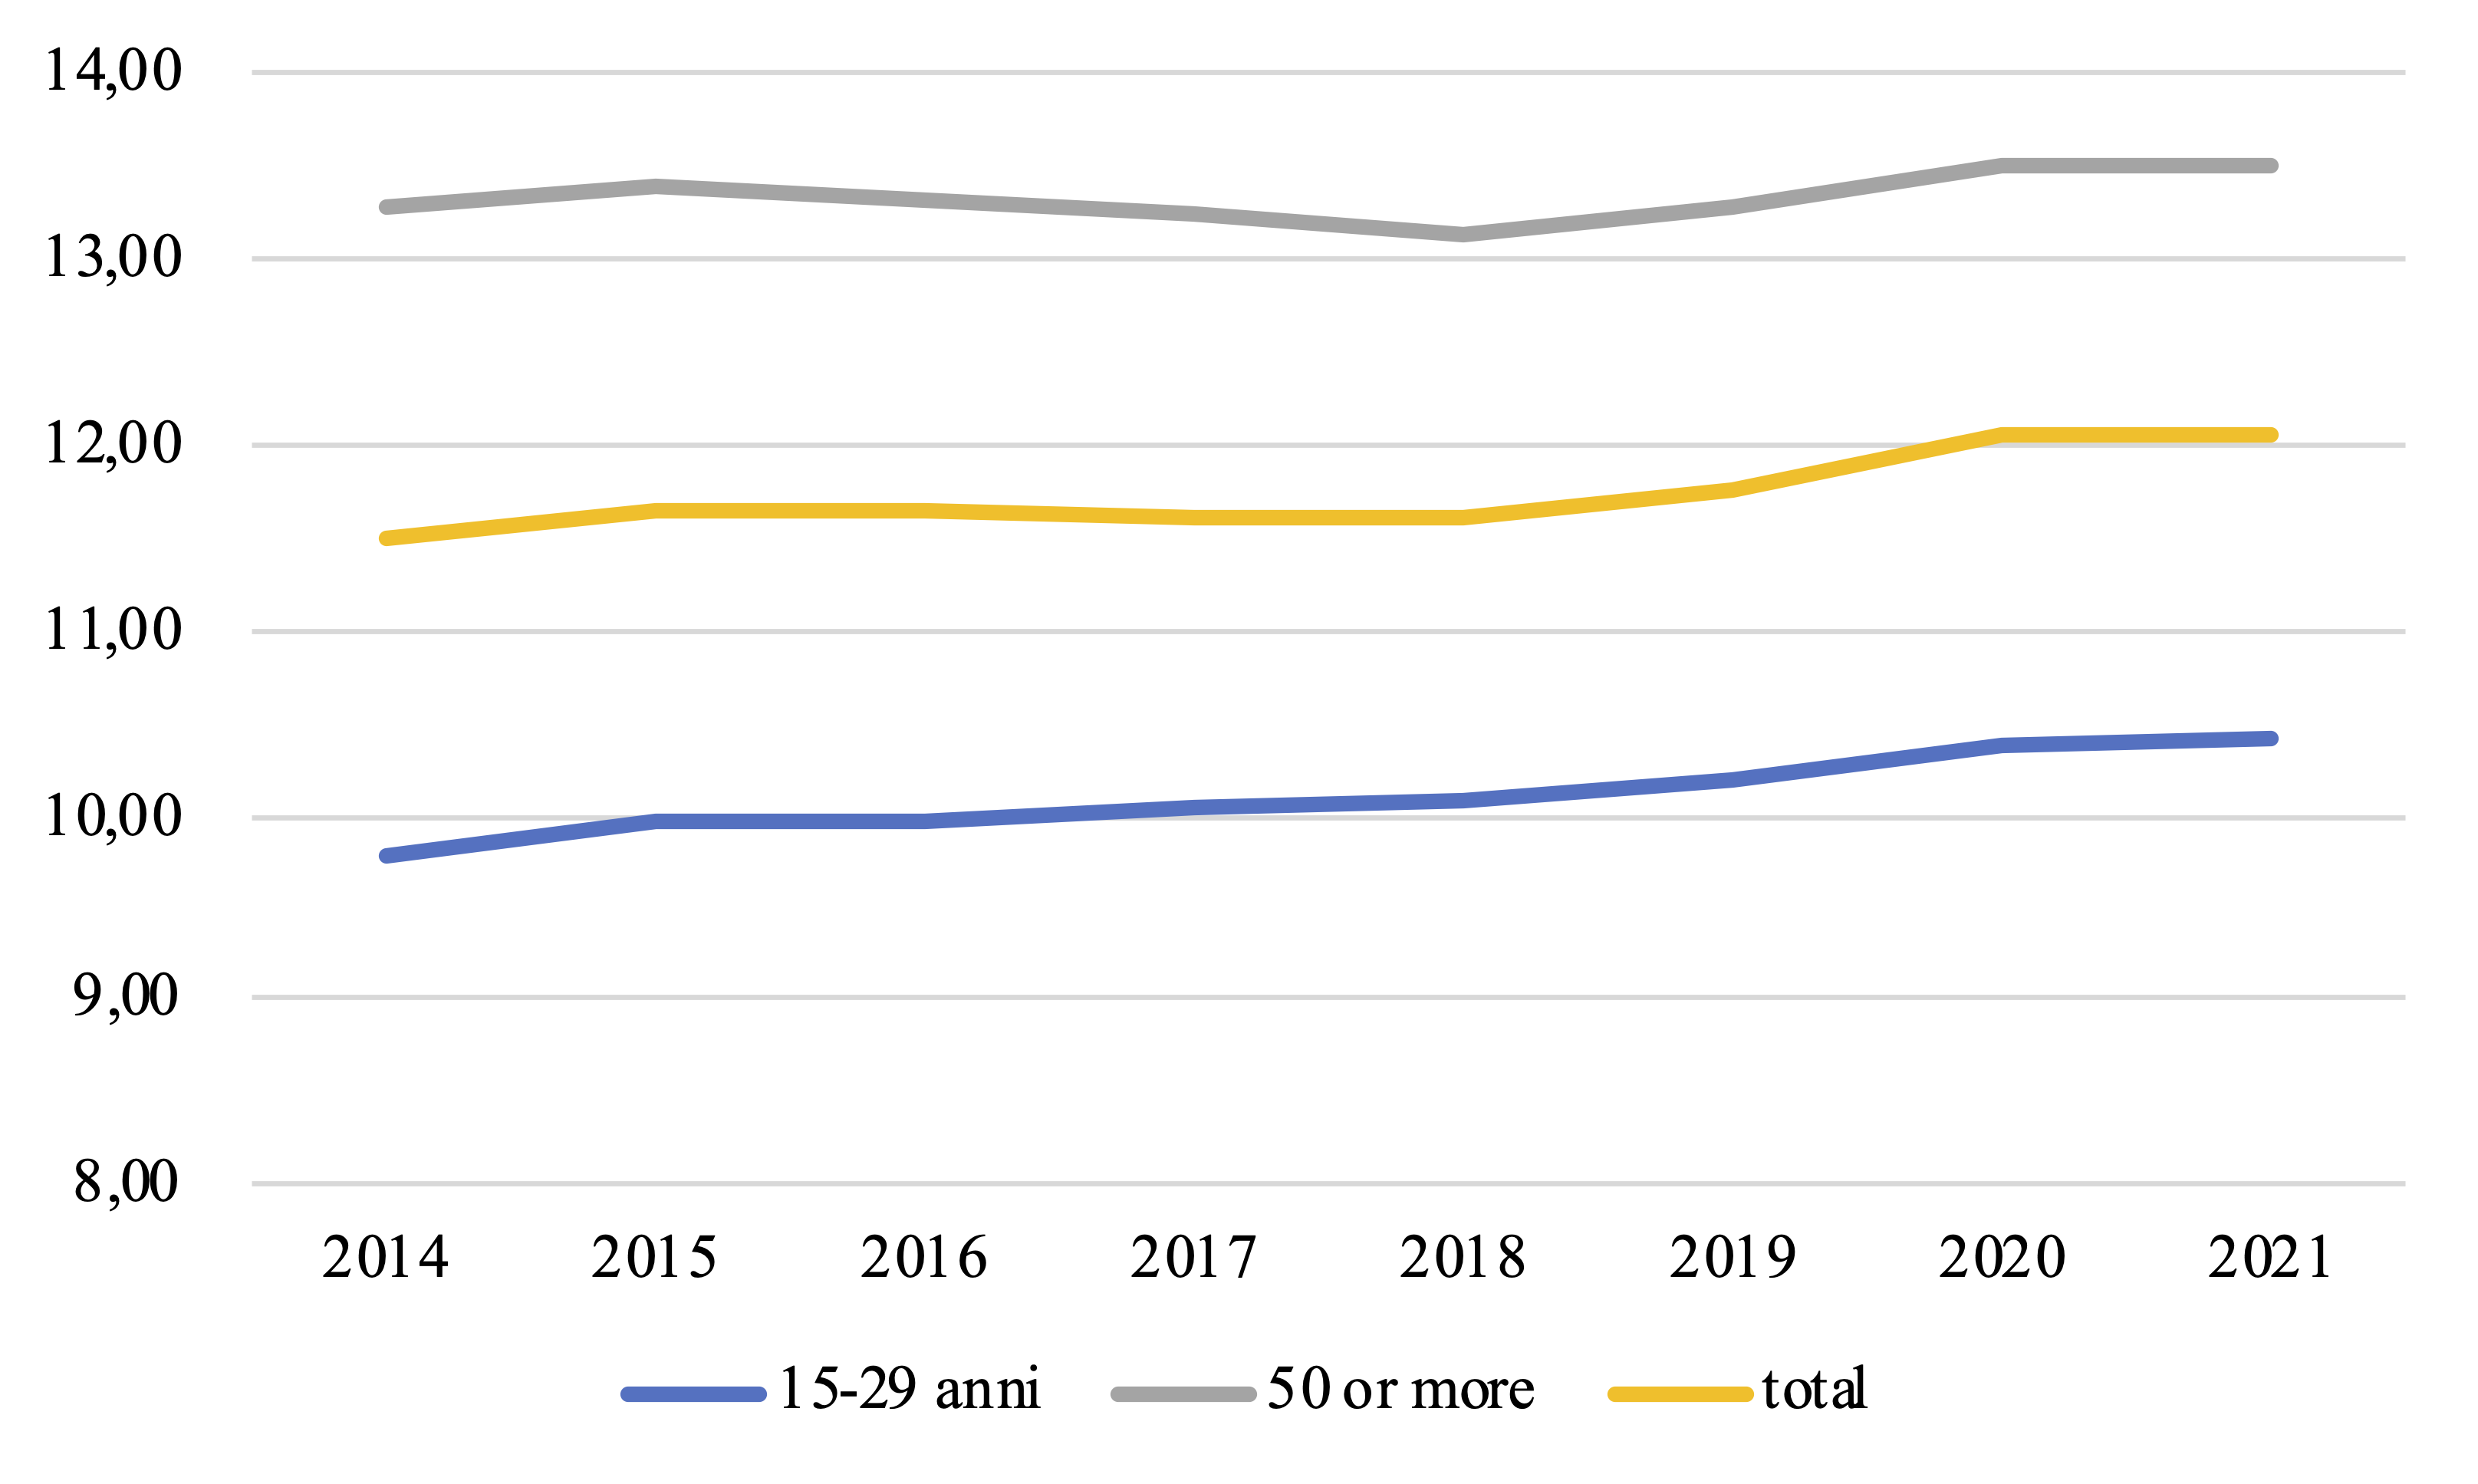
\includegraphics[width=\textwidth]{./images/hourly-wage-age.png}
		\end{center}
			\caption{Hourly wage in euros}
	\end{minipage}
	\begin{minipage}[b]{0.5\textwidth}
		\begin{center}
			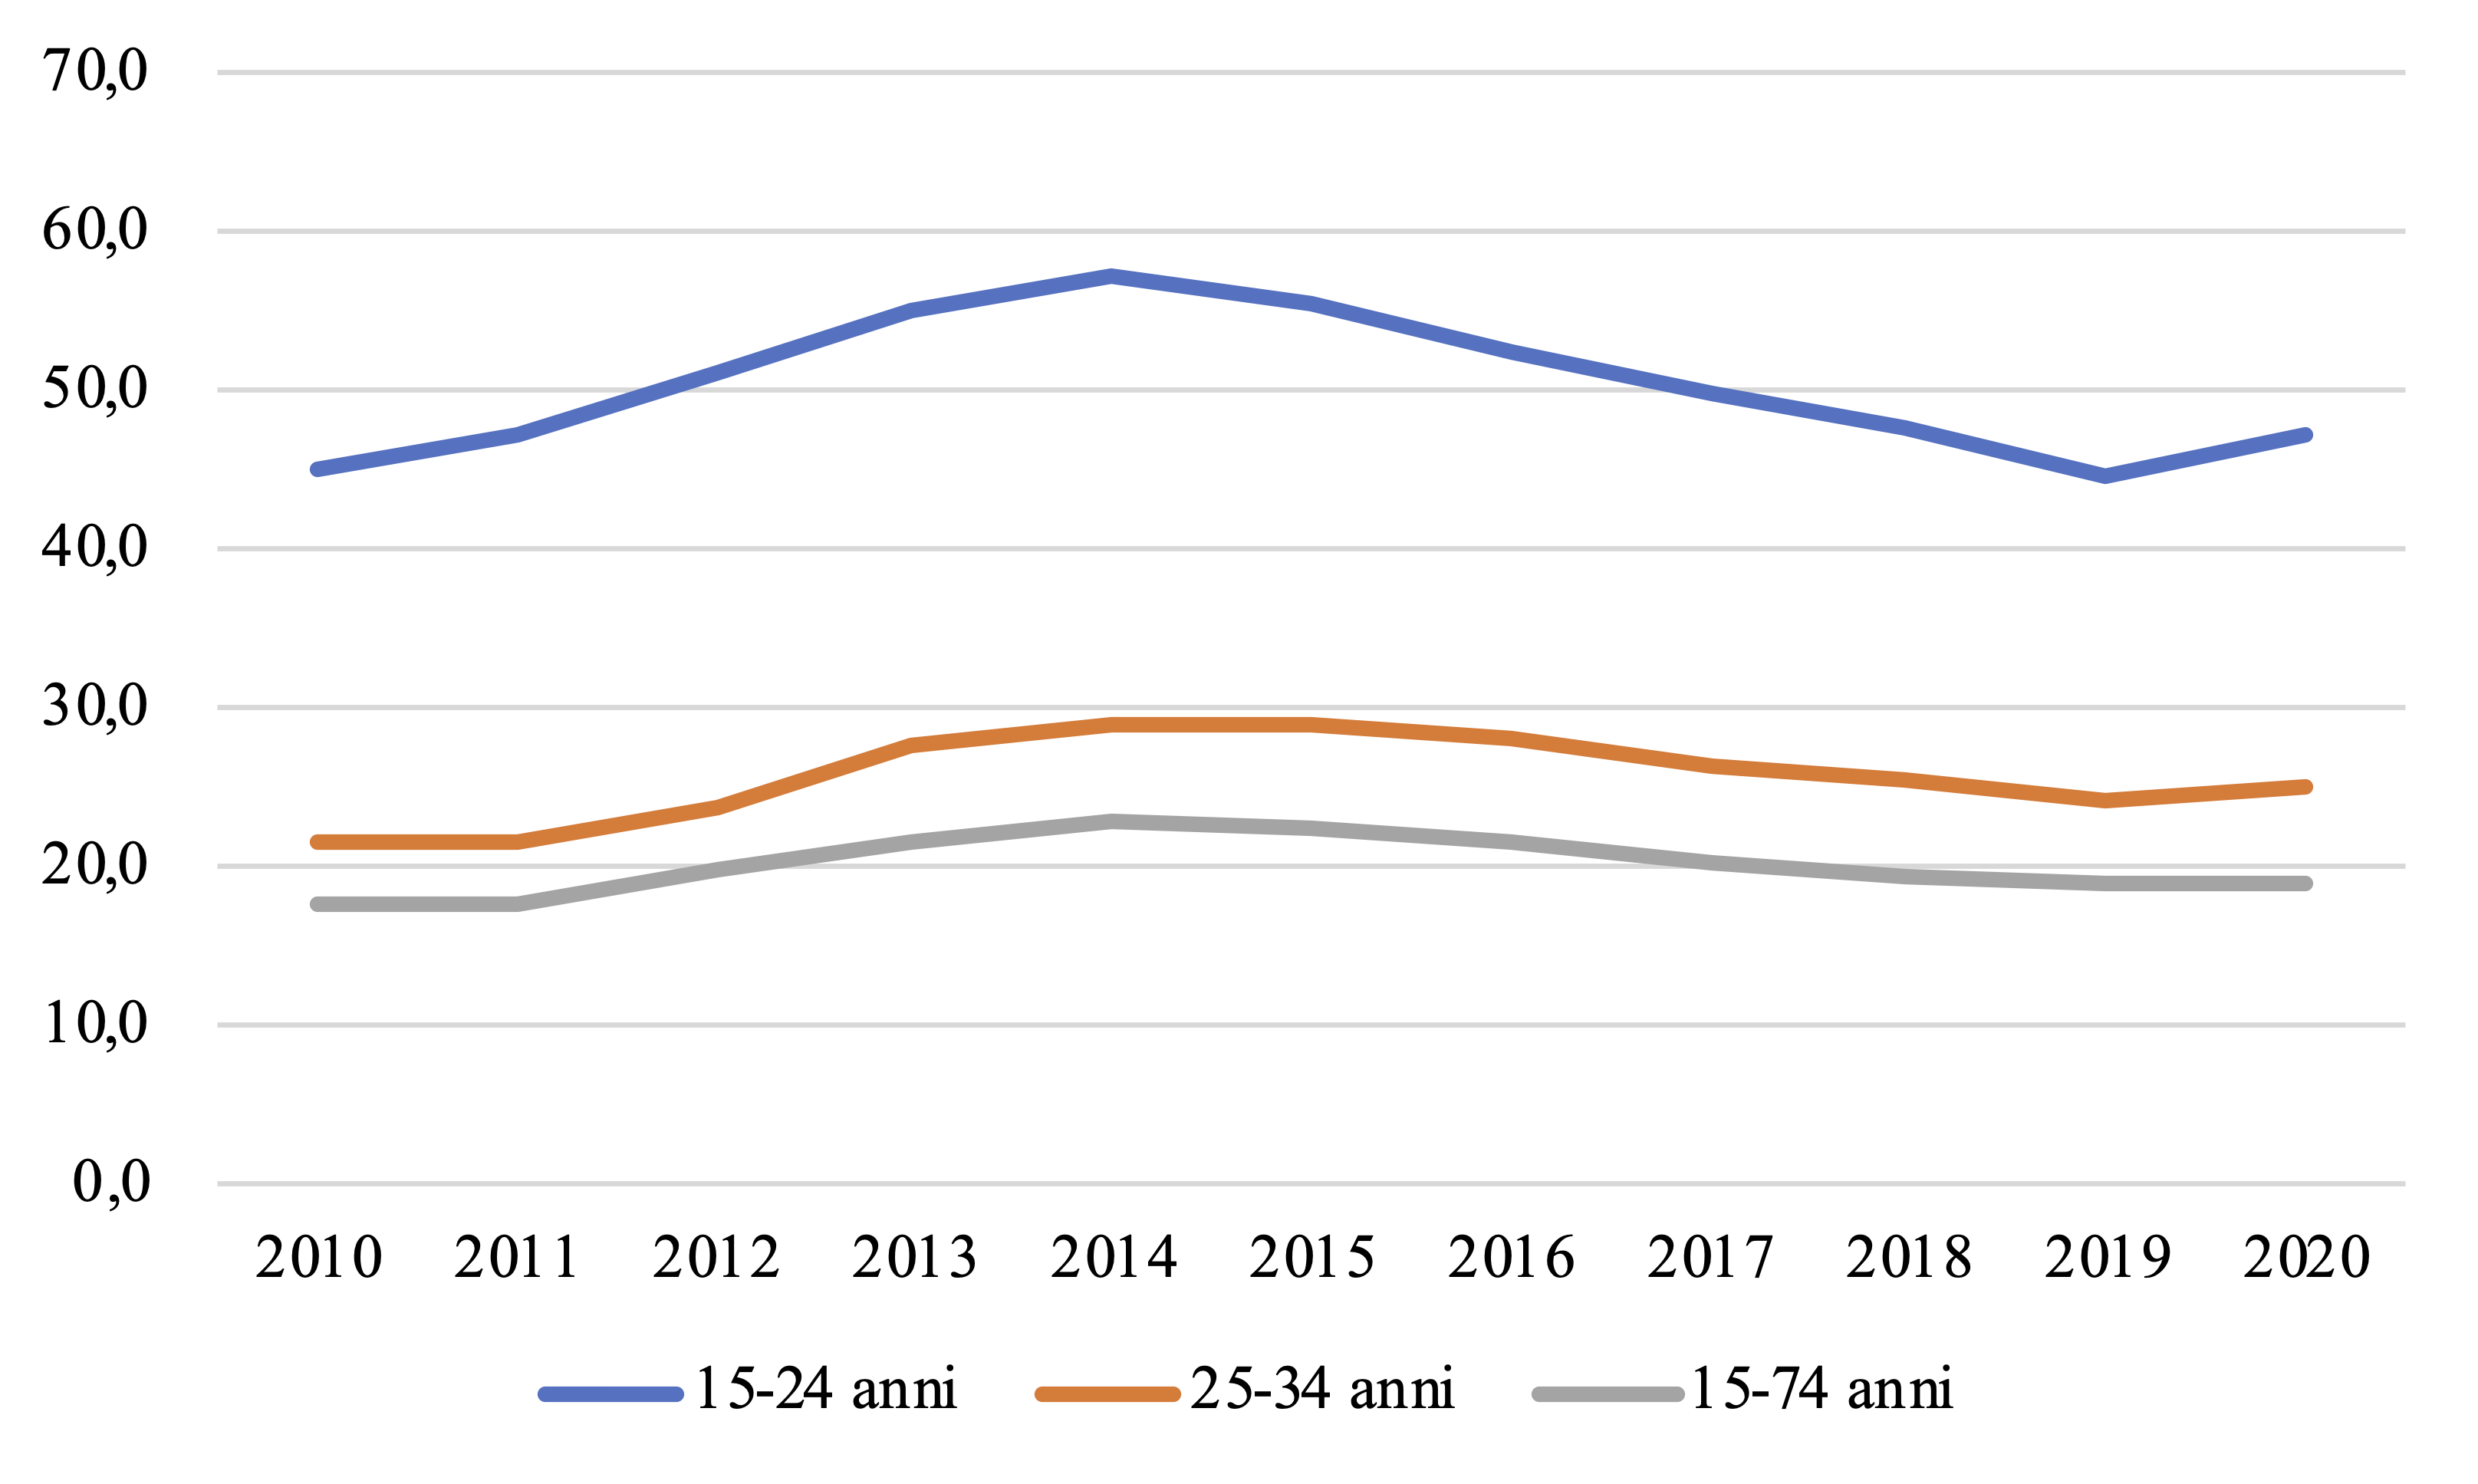
\includegraphics[width=\textwidth]{./images/non-participation-age.png}
		\end{center}
			\caption{Non participation rate}
	\end{minipage}
\end{figure}

\begin{figure}
	\begin{minipage}[b]{0.5\textwidth}
		\begin{center}
			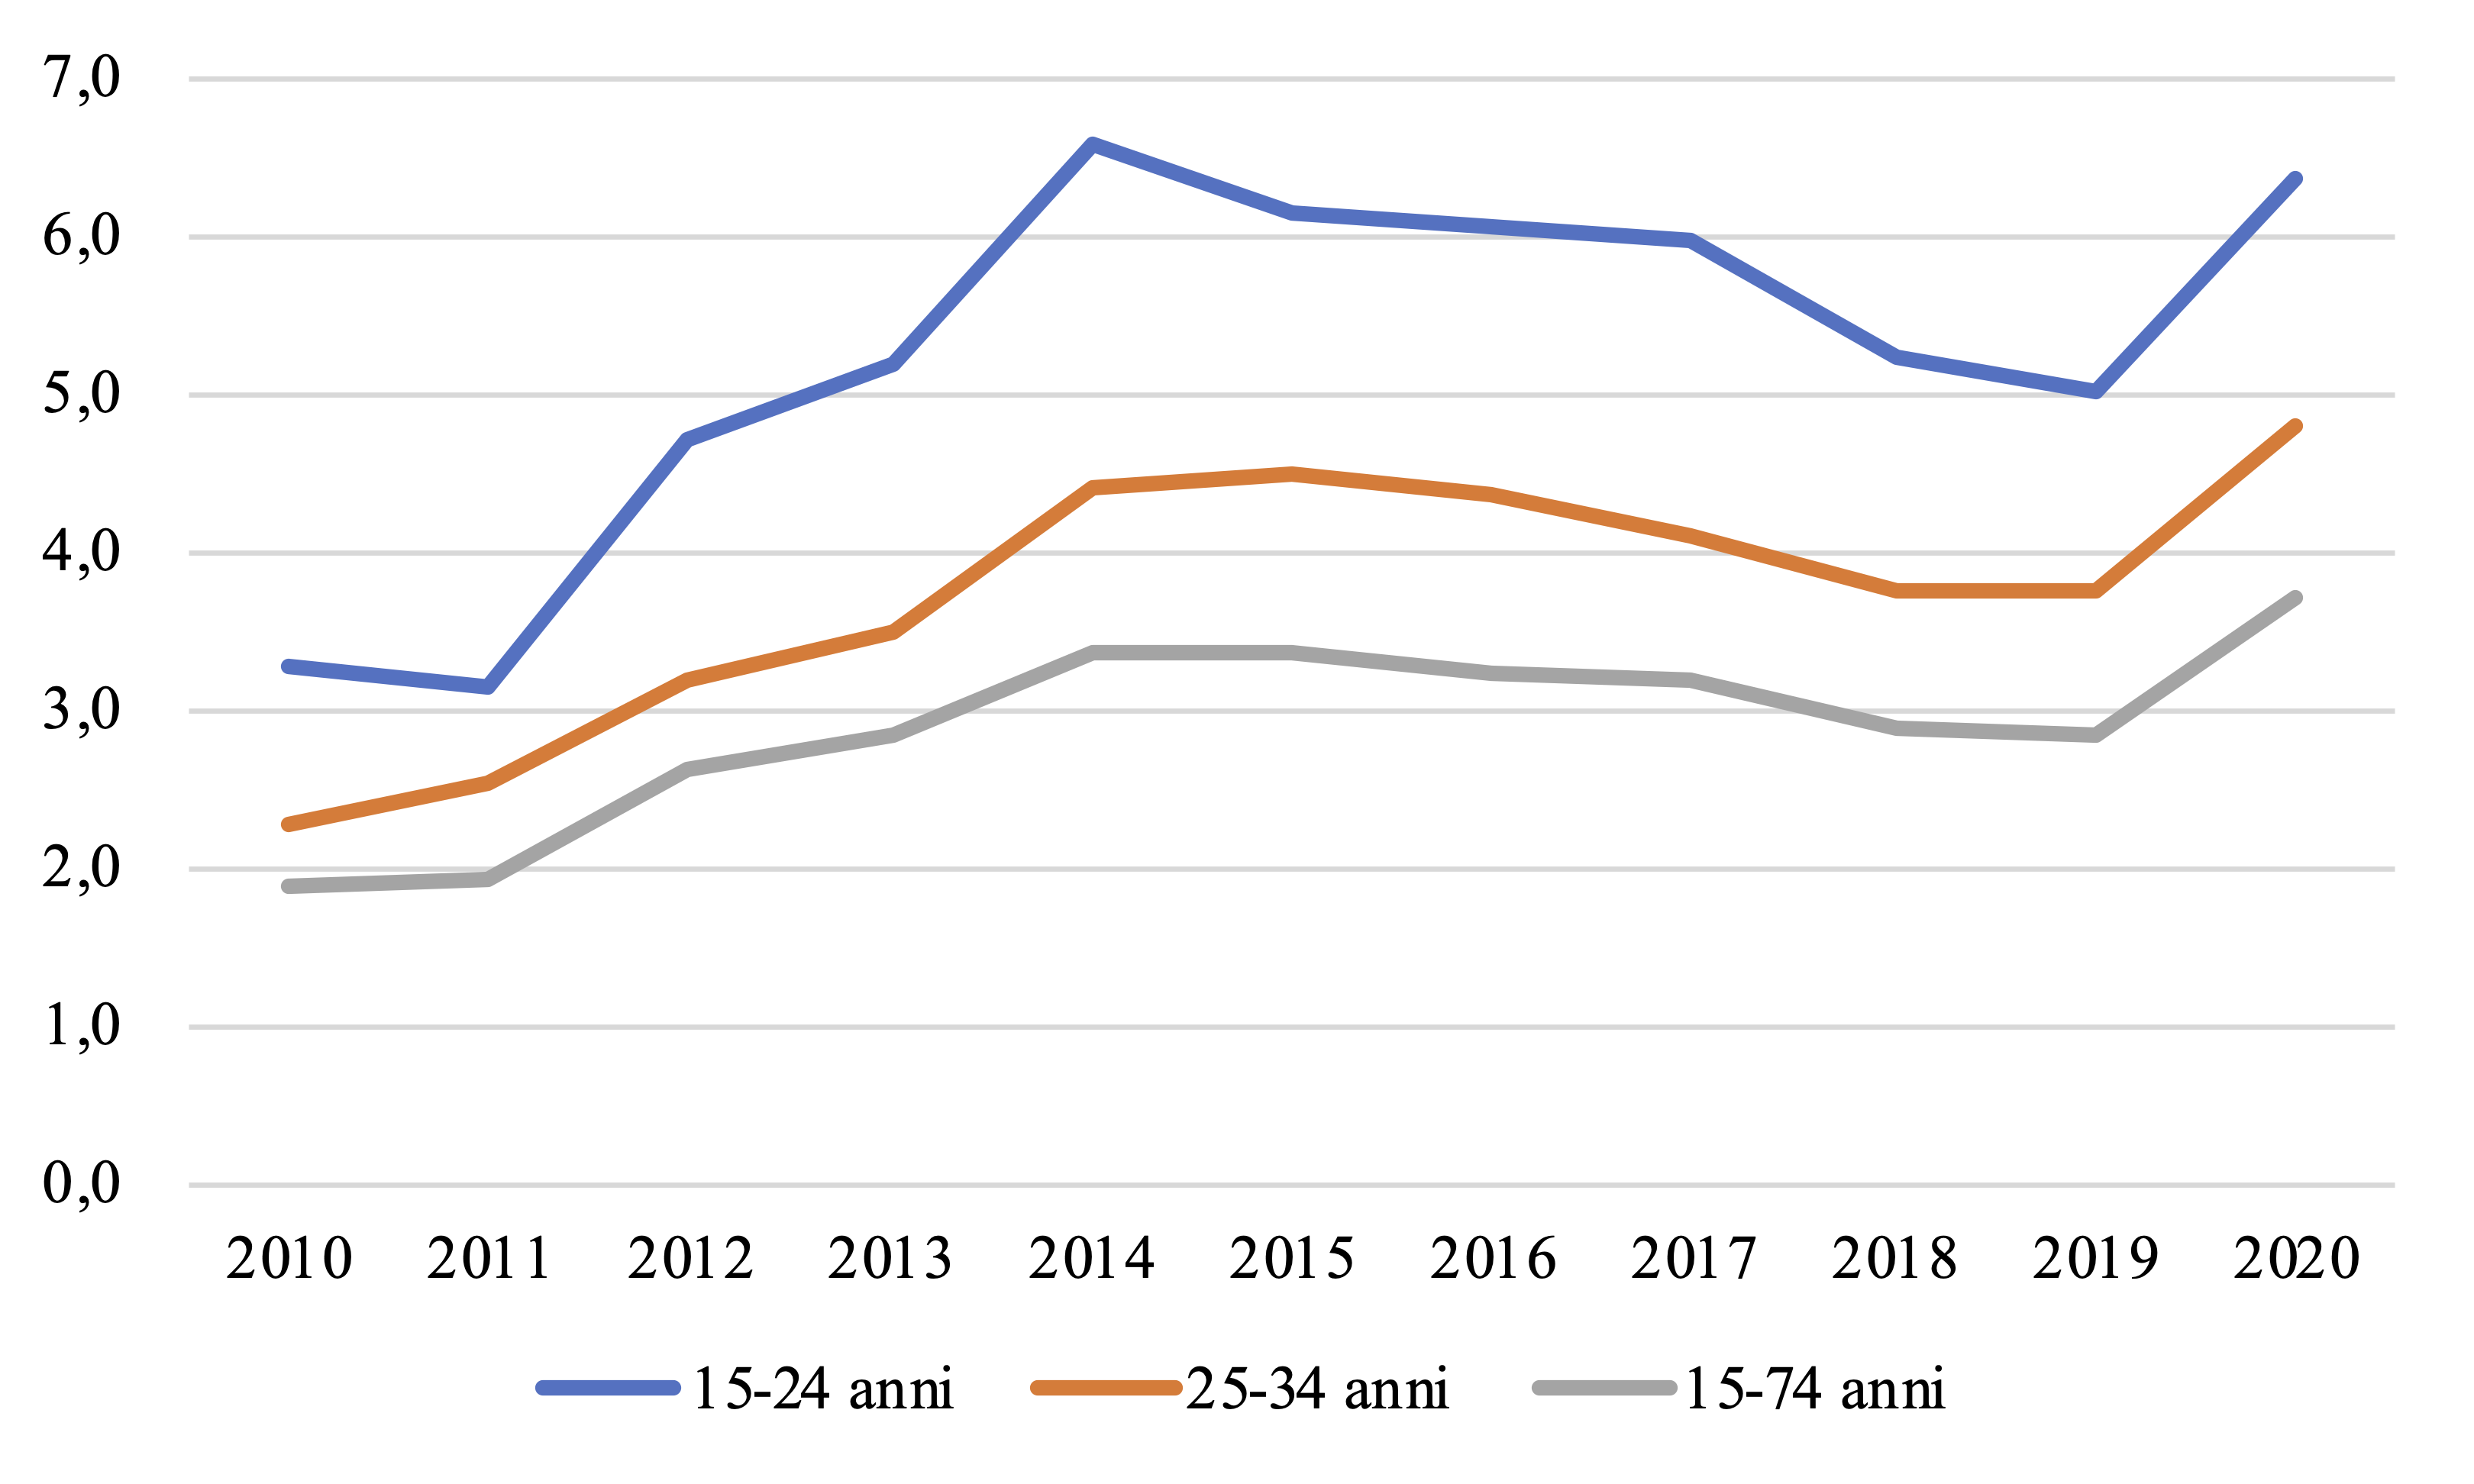
\includegraphics[width=\textwidth]{./images/underemployment-rate-age.png}
		\end{center}
			\caption{Underemployment rate}
	\end{minipage}
	\begin{minipage}[b]{0.5\textwidth}
		\begin{center}
			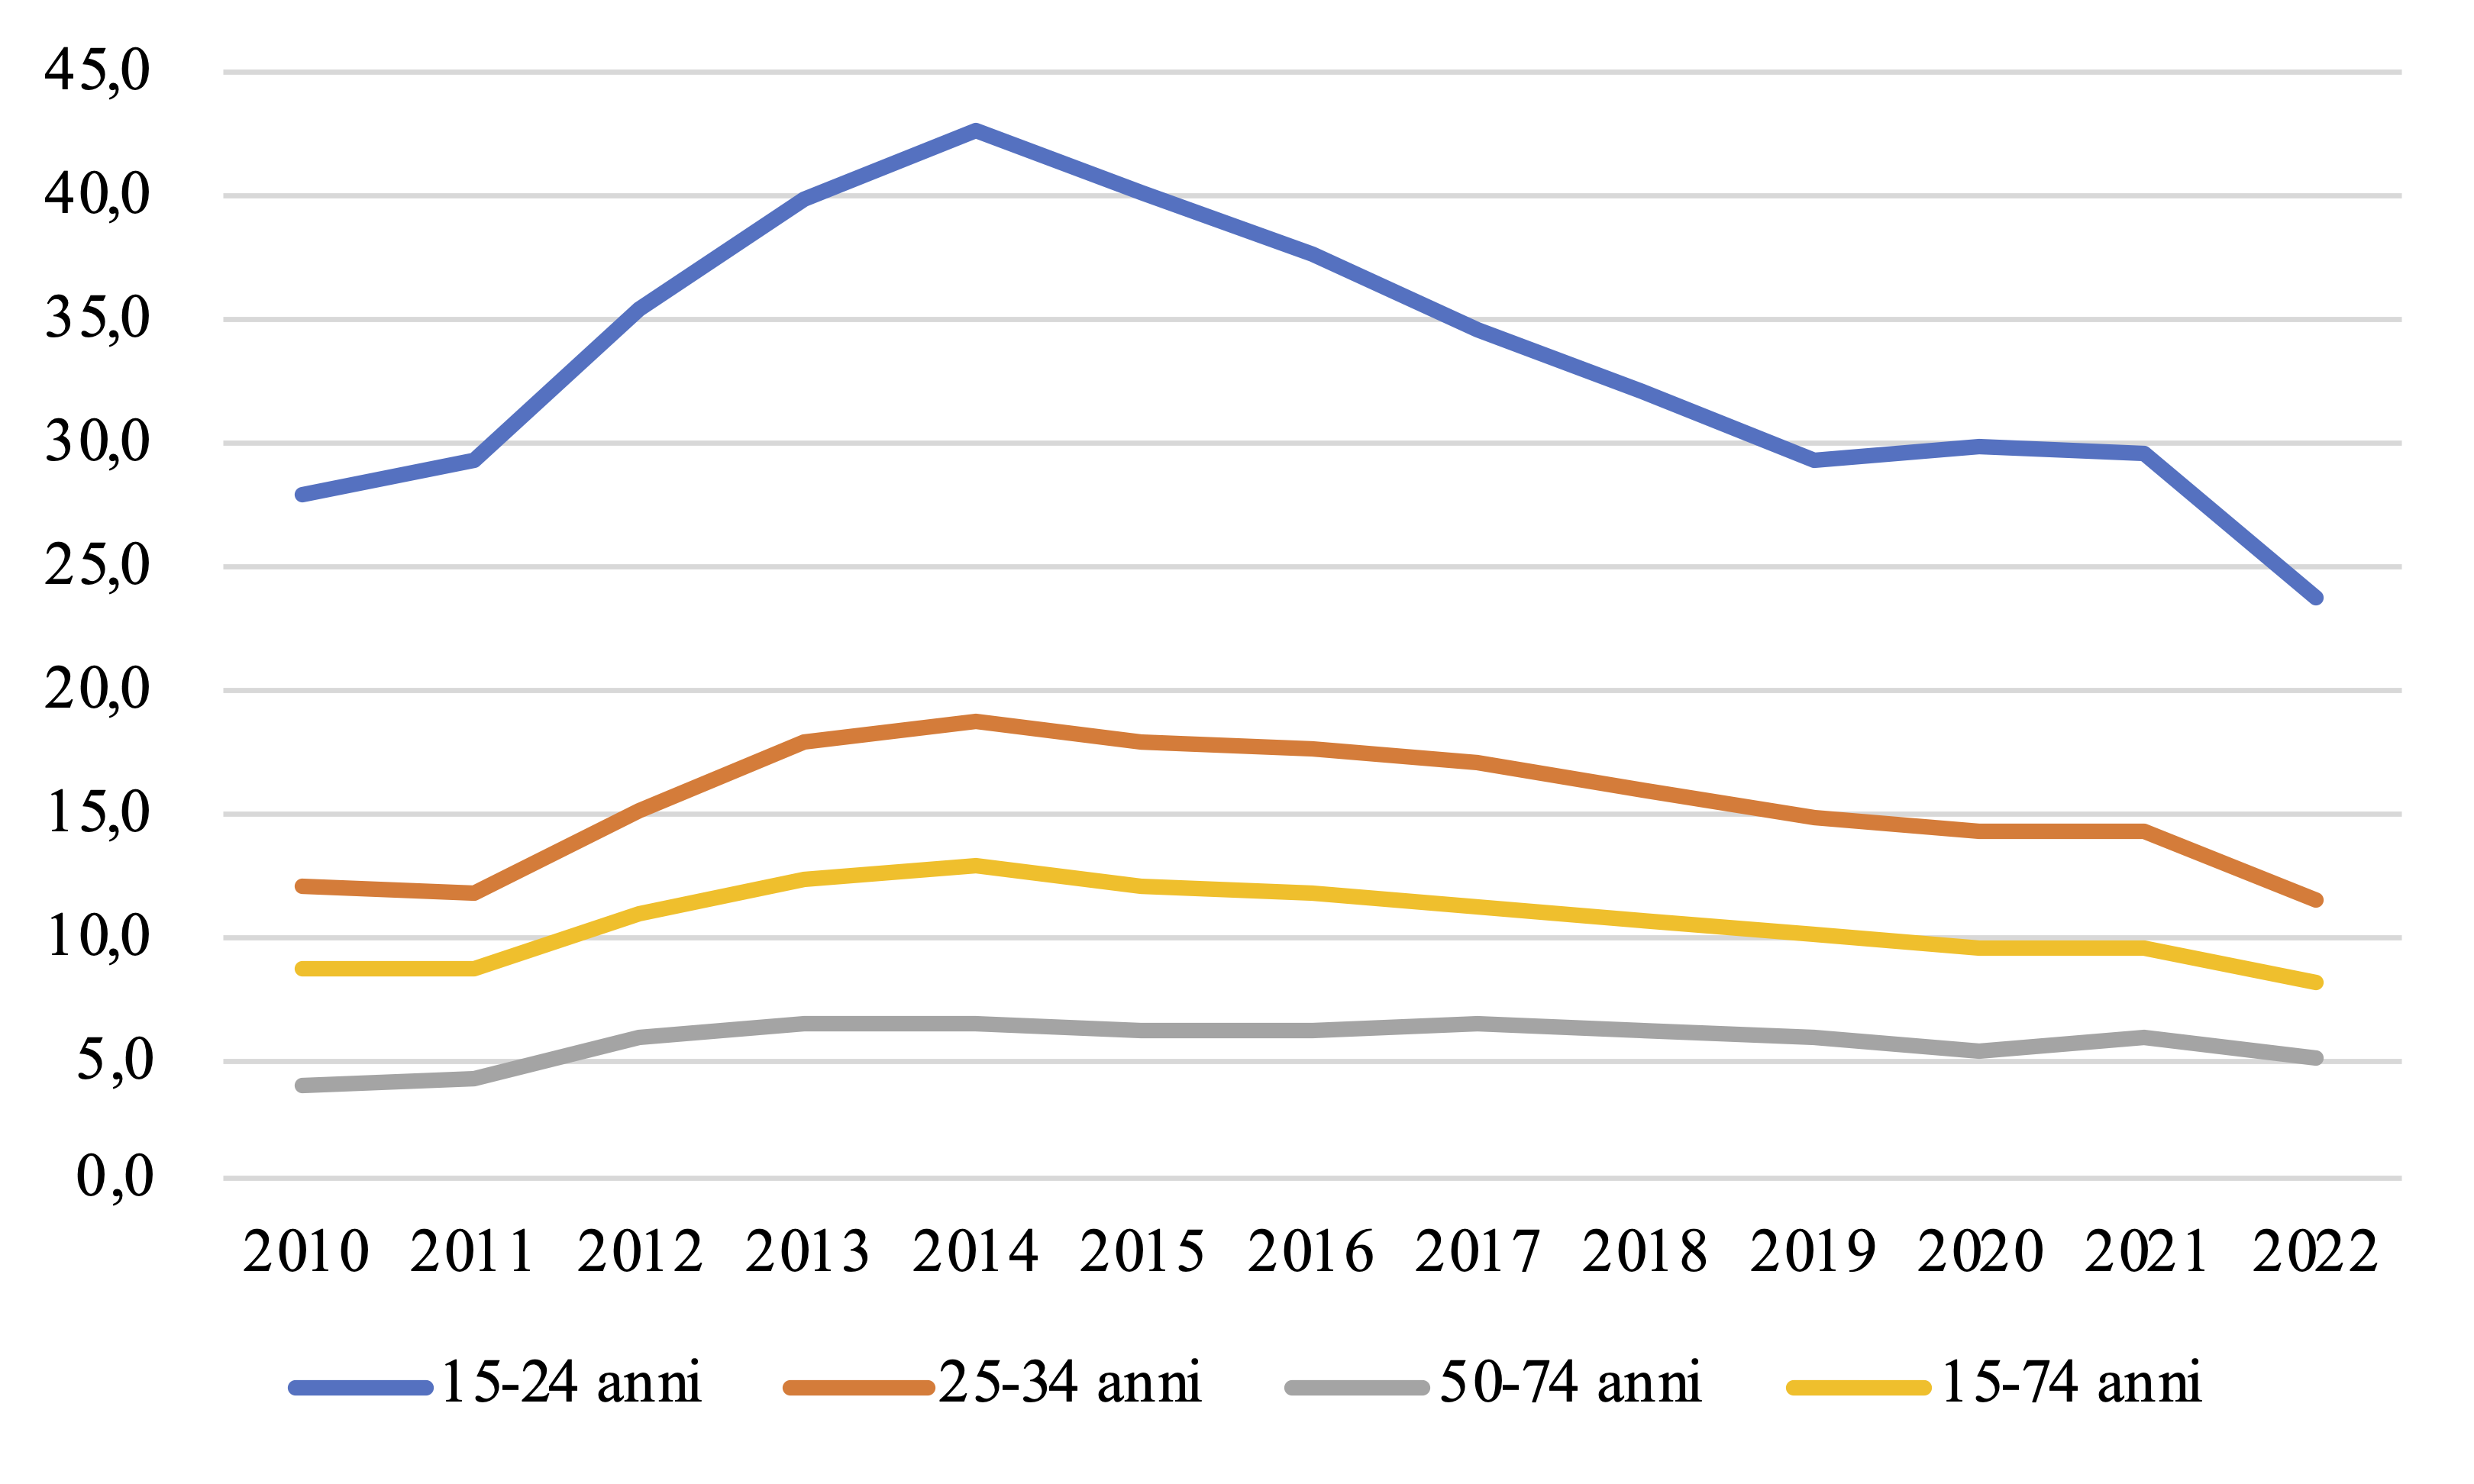
\includegraphics[width=\textwidth]{./images/unemployment-rate-age.png}
		\end{center}
			\caption{Unemployment rate}
	\end{minipage}
\end{figure}

%\begin{figure}
%\begin{center}
%	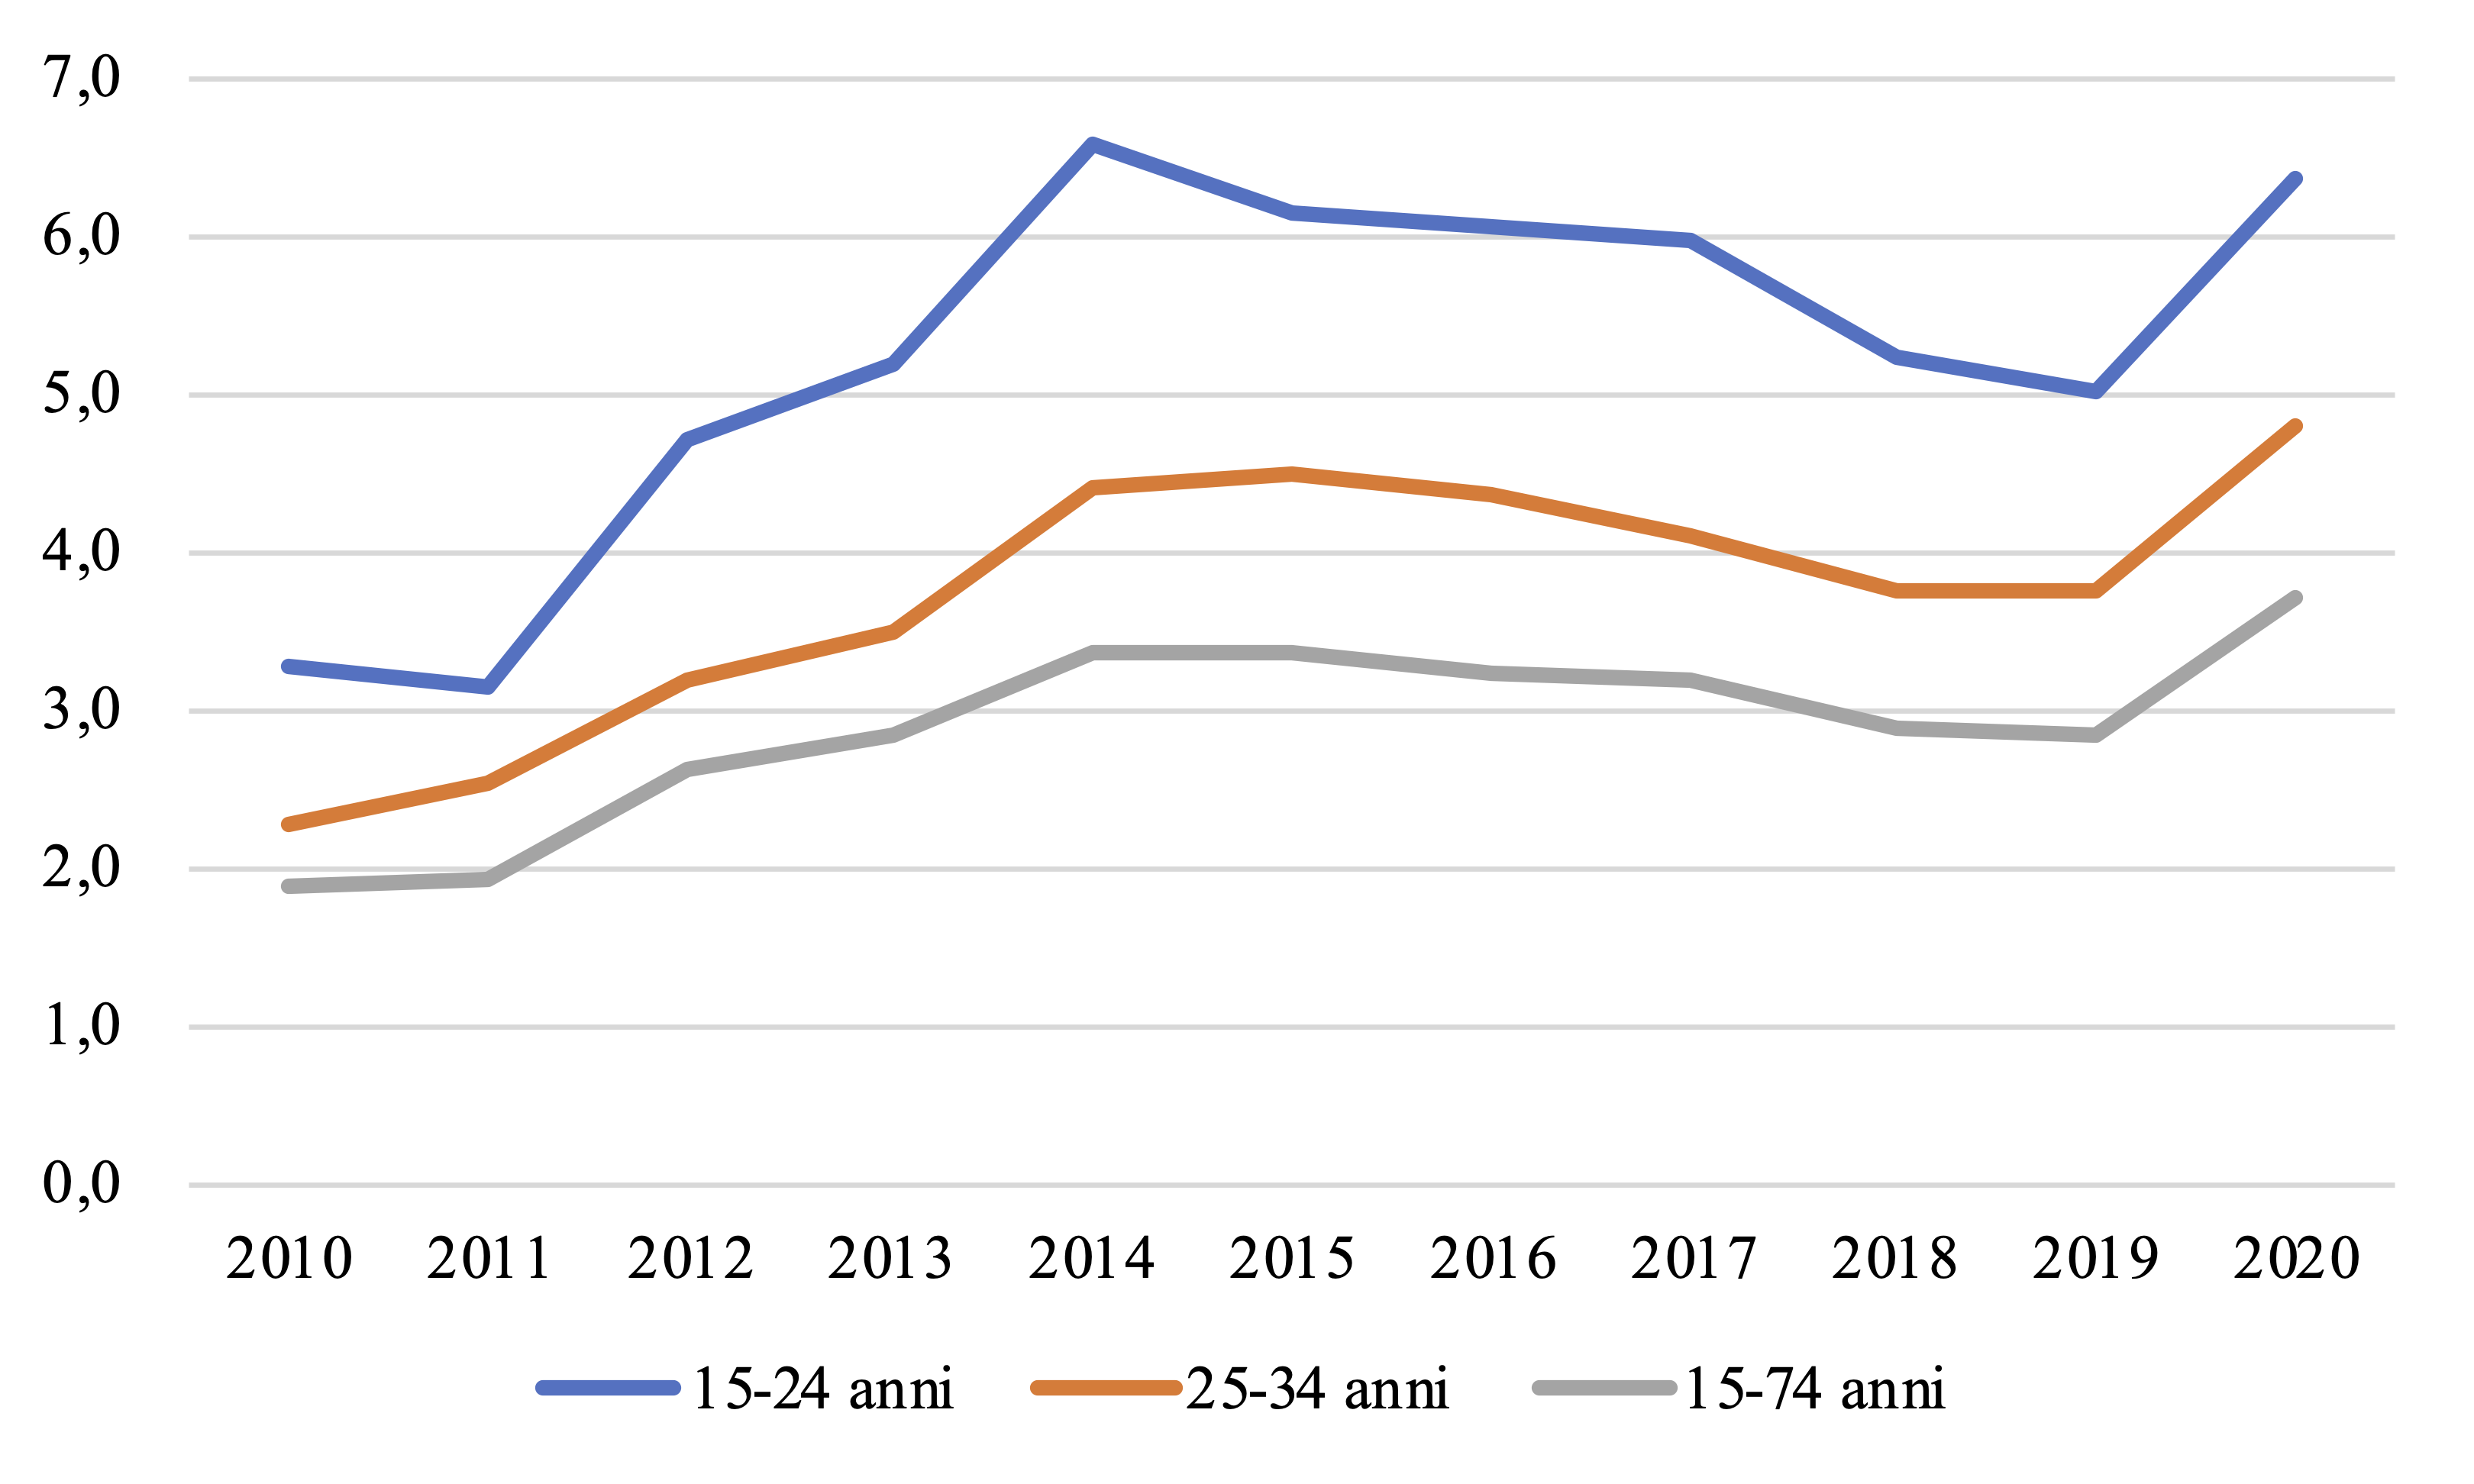
\includegraphics[width=0.7\textwidth]{./images/underemployment-rate-age.png}
%\end{center}
%	\caption{Underemployment rate}
%\end{figure}
%
%\begin{figure}
%\begin{center}
%	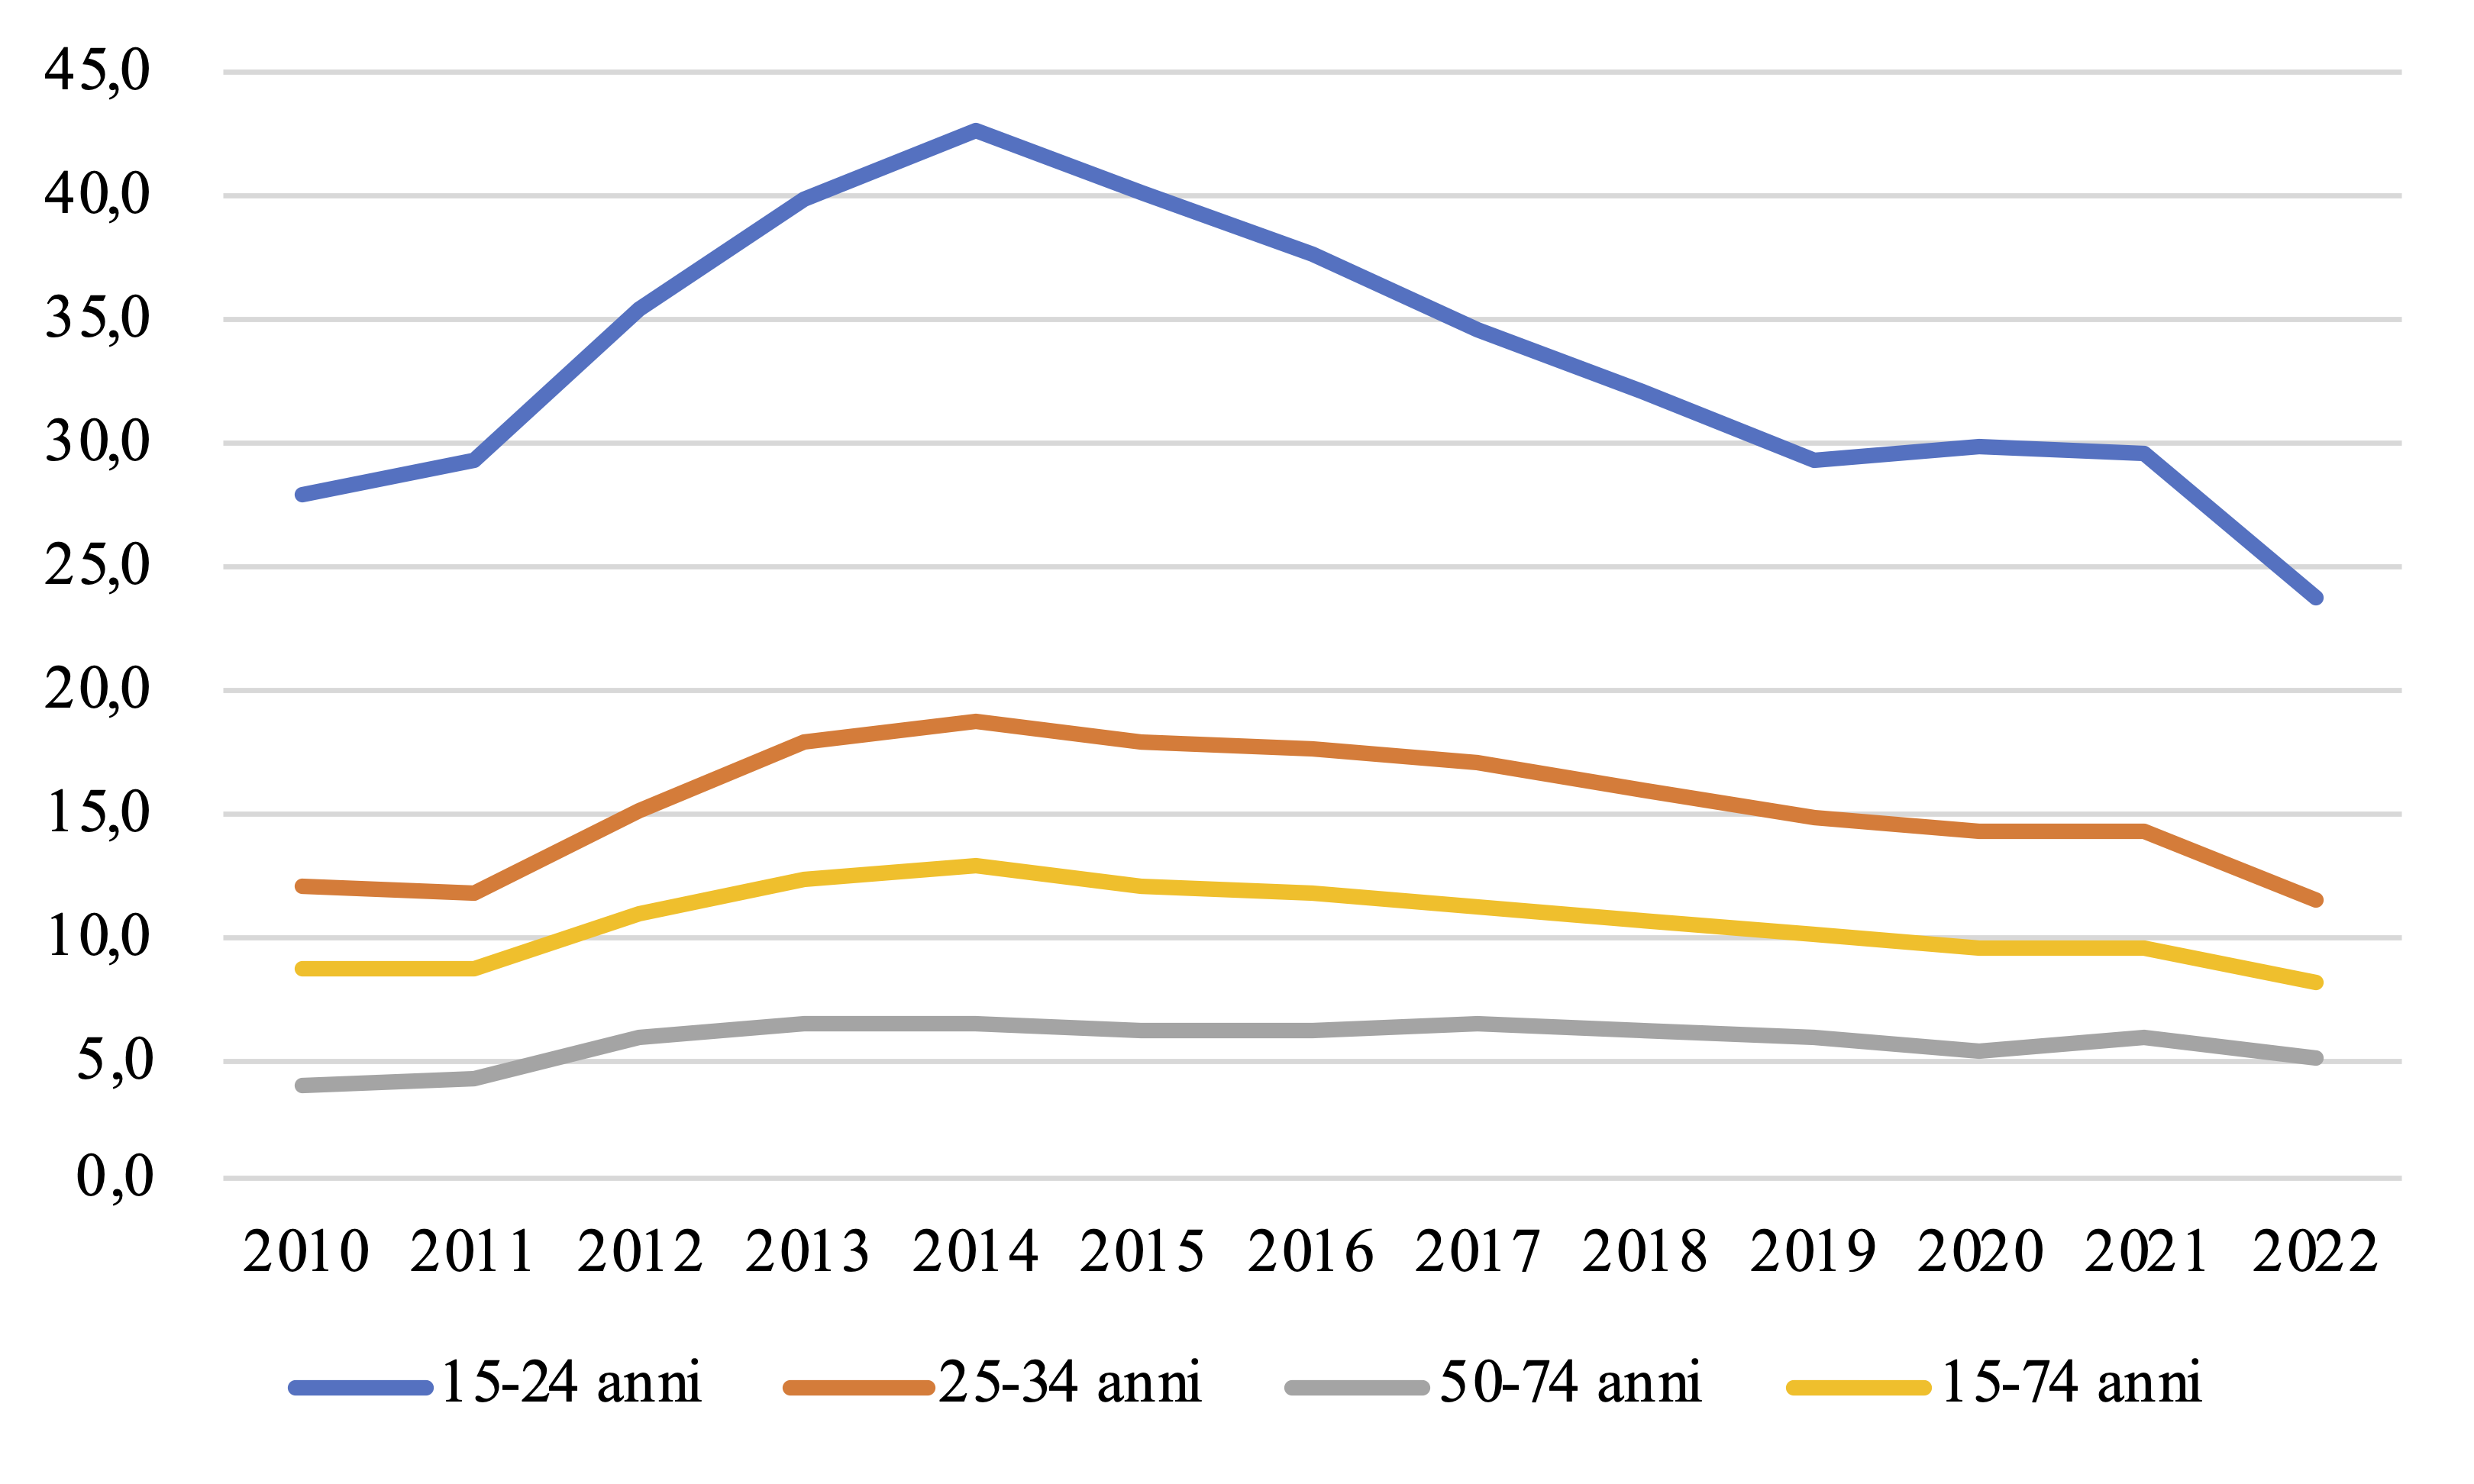
\includegraphics[width=14cm]{./images/unemployment-rate-age.png}
%\end{center}
%	\caption{Unemployment rate}
%\end{figure}

The percentage of people employed in between the ages 55 and 64 is 55\% in Italy. This may seem a good value but it is below the EU's 60.4\% \cite{eurostat2024employment}. In the case of older workers after a crisis or a period of recession, the time it takes to find a job grows more than that for other age groups, thus, they remain unemployed for a longer period of time. Moreover, Italians tend to work for a longer time due to an increase in the age required to access a pension, this means that there is less turnover. This has an impact on both young and old Italians. Another factor that has a strong effect on future employment of workers is their previous employment history. This makes it harder for older workers that have a bad employment history to break the cycle of low paying jobs. This shows that unemployment not only has a negative effect due to a person not being able to earn income but by also negatively affecting future employment opportunities. This effect is even further amplified by the fact that high skilled jobs tend to give workers a higher job security \cite{geroldi2013lavoro}. 

\end{spacing}

\subsection{Gender}

\begin{spacing}{1.5}

The average hourly wage for men in 2021 was €12.04 while the average hourly wage for women in the same year was €11.23. The gap between the two has diminished over time from 8.09\% to 7.03\% but one still remains. We could reduce the difference between men and women to only their wages but their are also many other factors in which they are affected differently and could affect their income. We should also try to understand why this difference exists.

The employment rate for women is lower than for men, 51.1\% and 69.2\% respectively in 2022. The employment rate has gone up over time for both age groups but it has increased at a faster rate for women than for men, there has been an increase of 3.6 percent points in the employment rate for men since 2010 while there was an increase of 11.35 points for women. In some factors men are more vulnerable to the effects of a crisis than women are. This can be seen by a reduction in the difference between the percentage of occupied men and women between 2008 and 2016 \cite{canal2018punto}. The rate of part time workers for men and for women in 2022 are 8.28\% and 31.78\% respectively. The rate of part time workers has increased over time for both groups but more significantly for women. The rate of part time workers for men has gone up from 5.48\% to 8.61\% from 2010 to 2020, while for women it increased from 28.92\% to 32.09\%. Another interesting fact is that the rate of full time workers has gone down for men while it remained stable for women in the same time period. For men, it decreased from 94.52\% to 91.39\%, and for women it decreased from 71.08\% to 67.91\% so the difference remained the same. Part time work during a crisis increases and it increases more for men than for women \cite{canal2018punto}. Part time work most of the time occurs due to not being able find a full time job. In 2020, of the men working part time, 74.2\% would have preferred a full time job and of the women working part time 61.1\% would have preferred a full time job. These rates have increased over time for both groups, for men in 2010 the value was 59.3\% and for women it was 46.1\%. The difference between the two groups has remained stable over time, being 13.1\% in 2010 and 13.1\% in 2020.

\begin{figure}
	\begin{minipage}[b]{0.5\textwidth}
		\begin{center}
			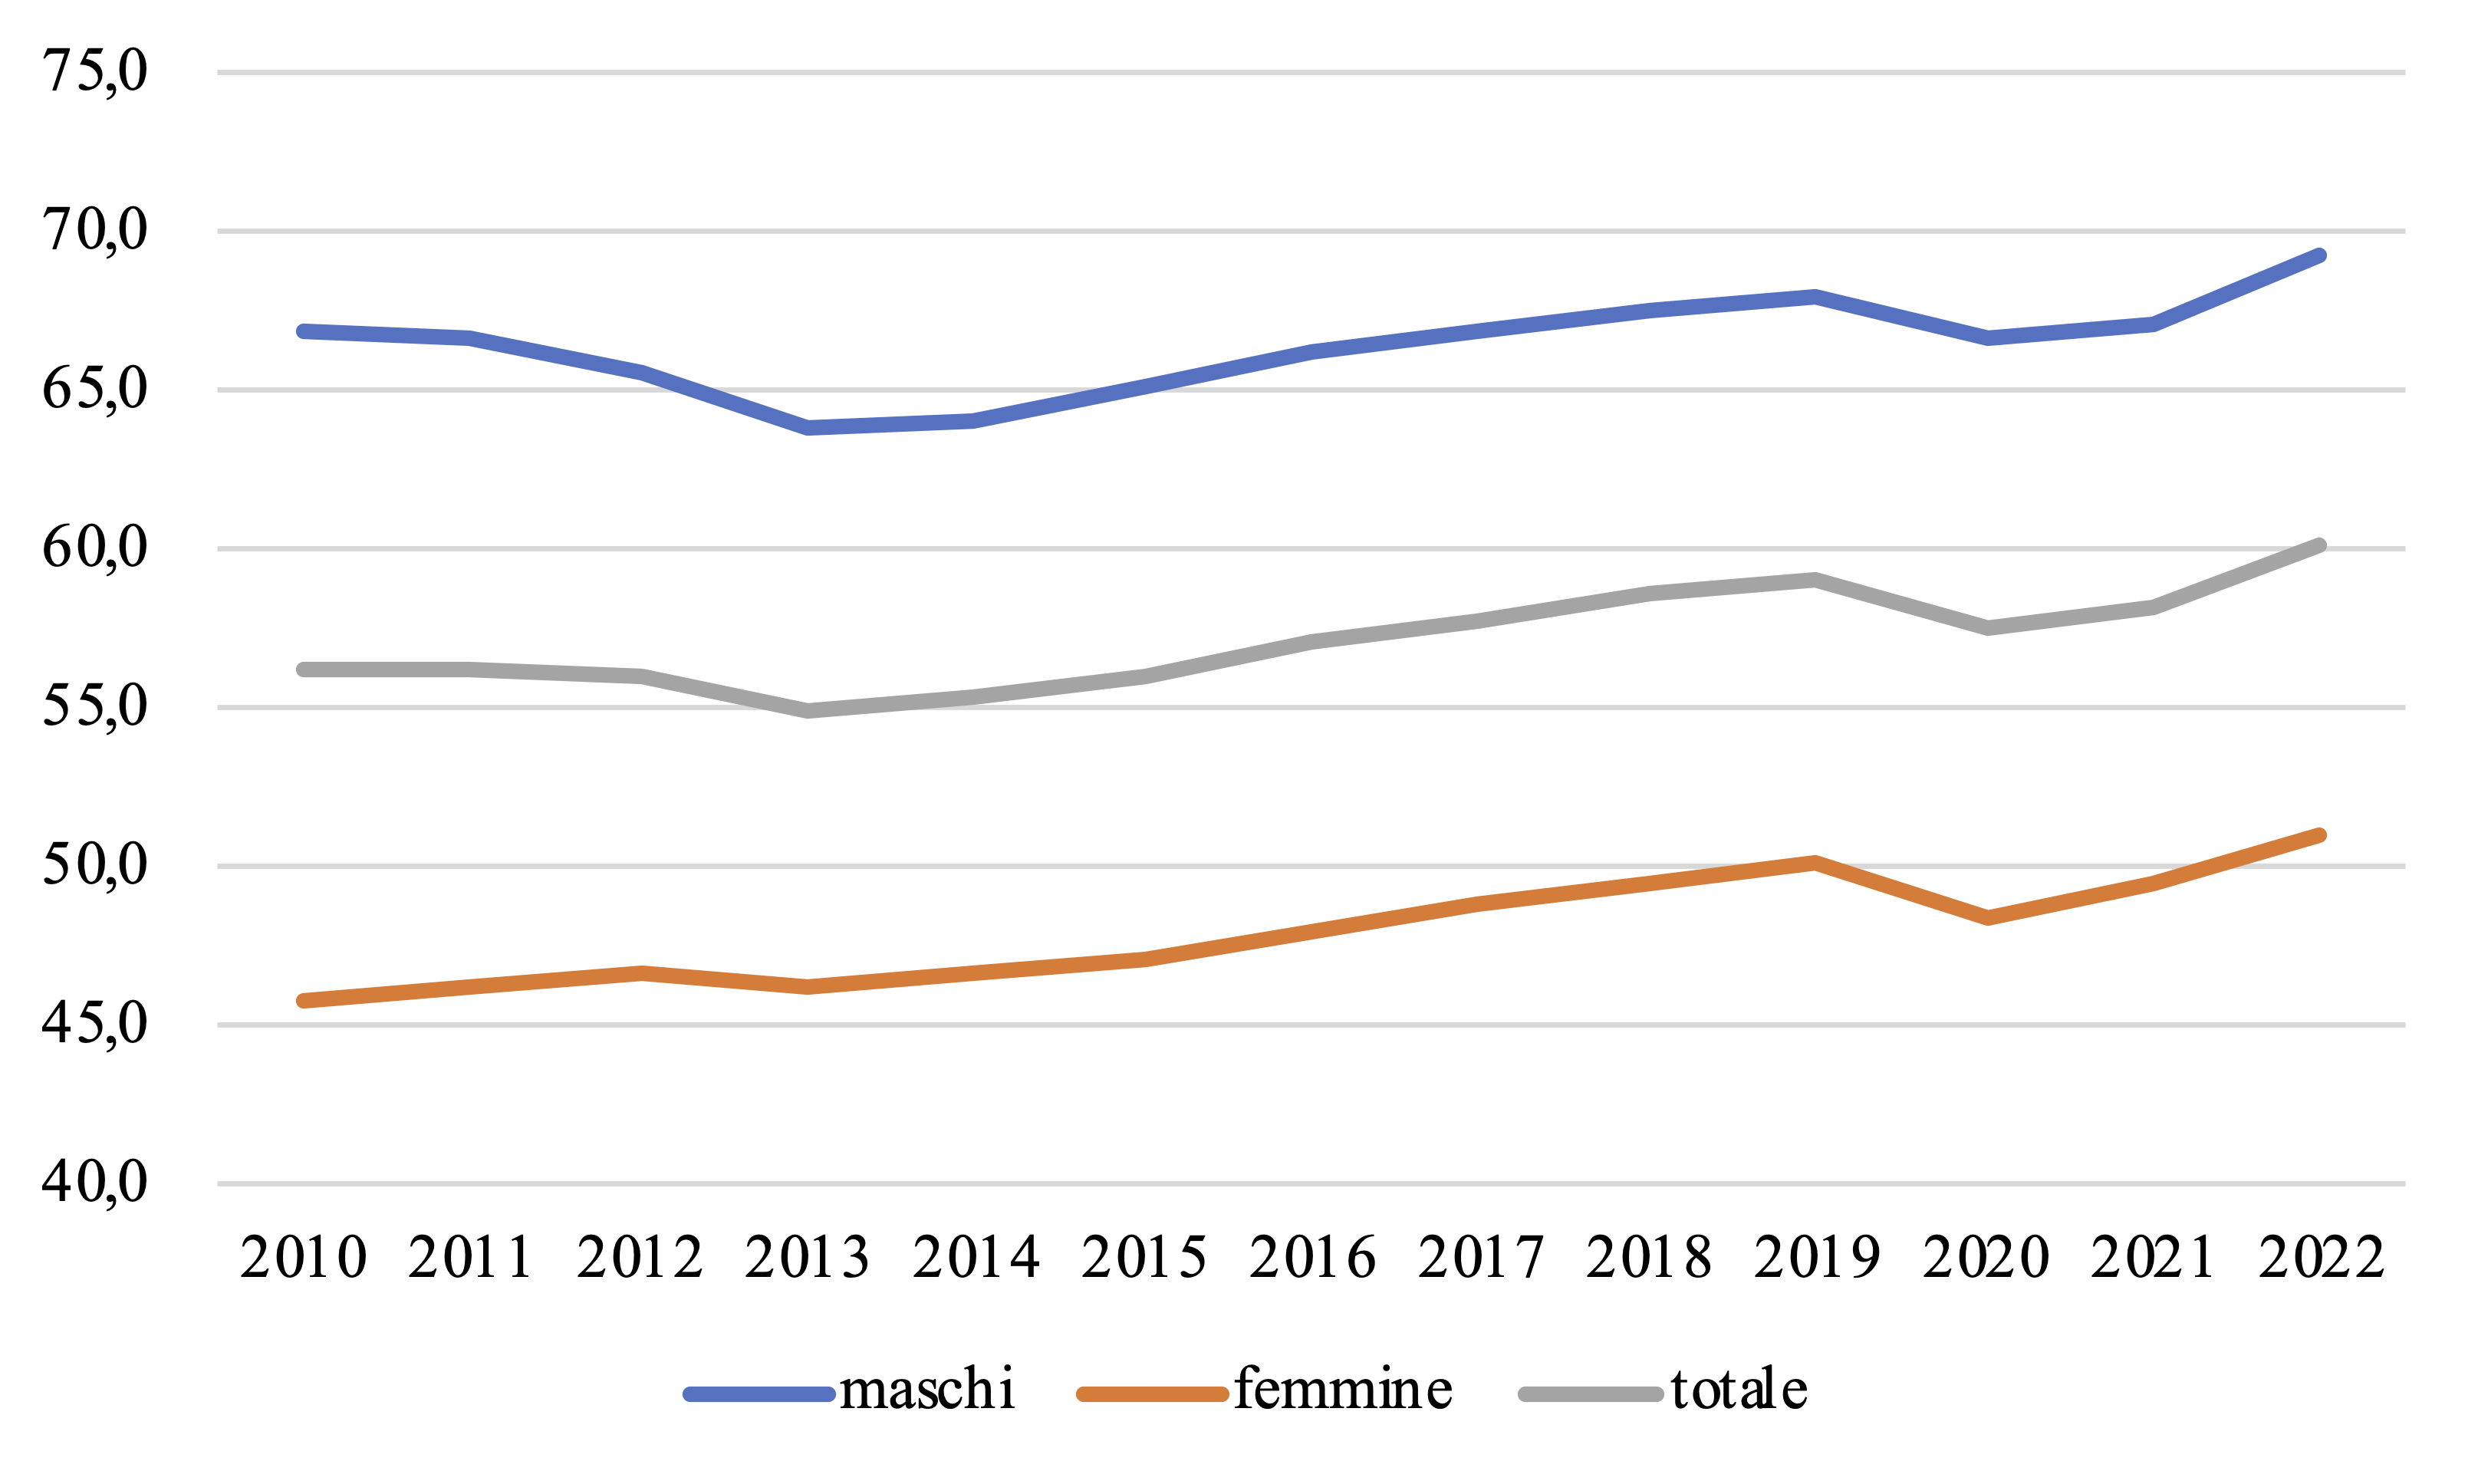
\includegraphics[width=\textwidth]{./images/employment-rate-gender.png}
		\end{center}
			\caption{Employment rate}
	\end{minipage}
	\begin{minipage}[b]{0.5\textwidth}
		\begin{center}
			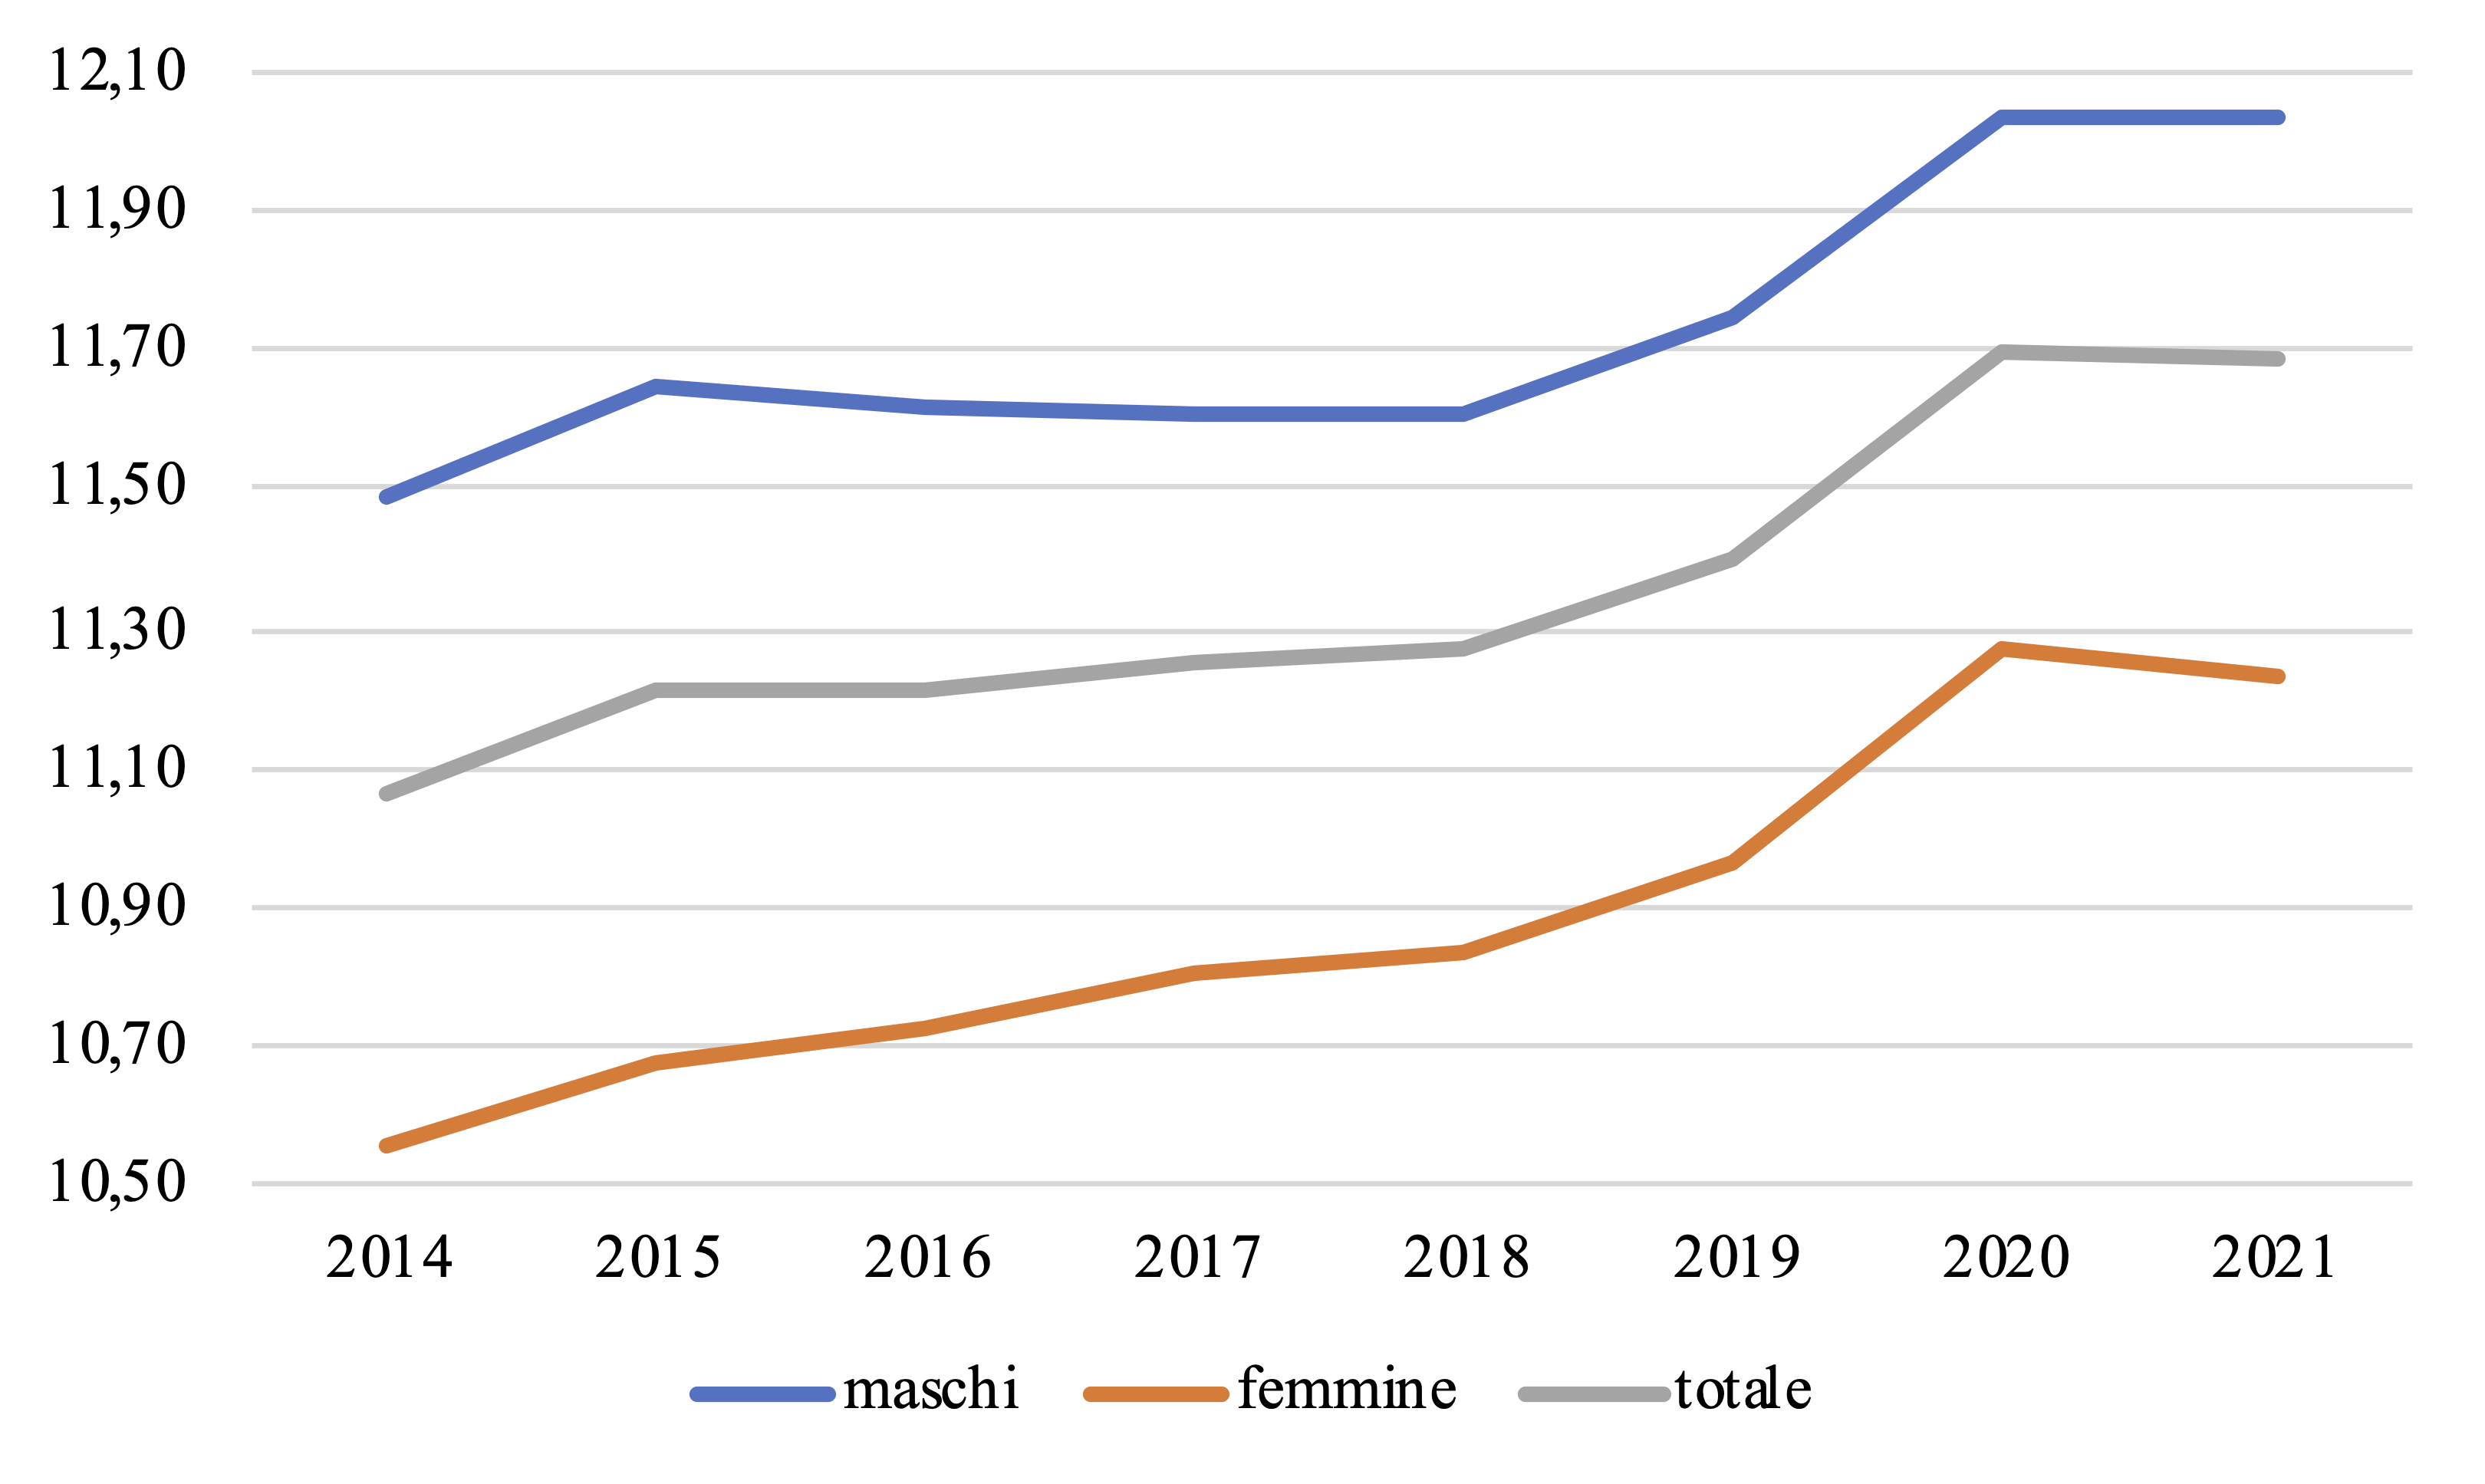
\includegraphics[width=\textwidth]{./images/hourly-wage-gender.png}
		\end{center}
			\caption{Hourly wage in euros}
	\end{minipage}
\end{figure}

\begin{figure}
	\begin{minipage}[b]{0.5\textwidth}
		\begin{center}
			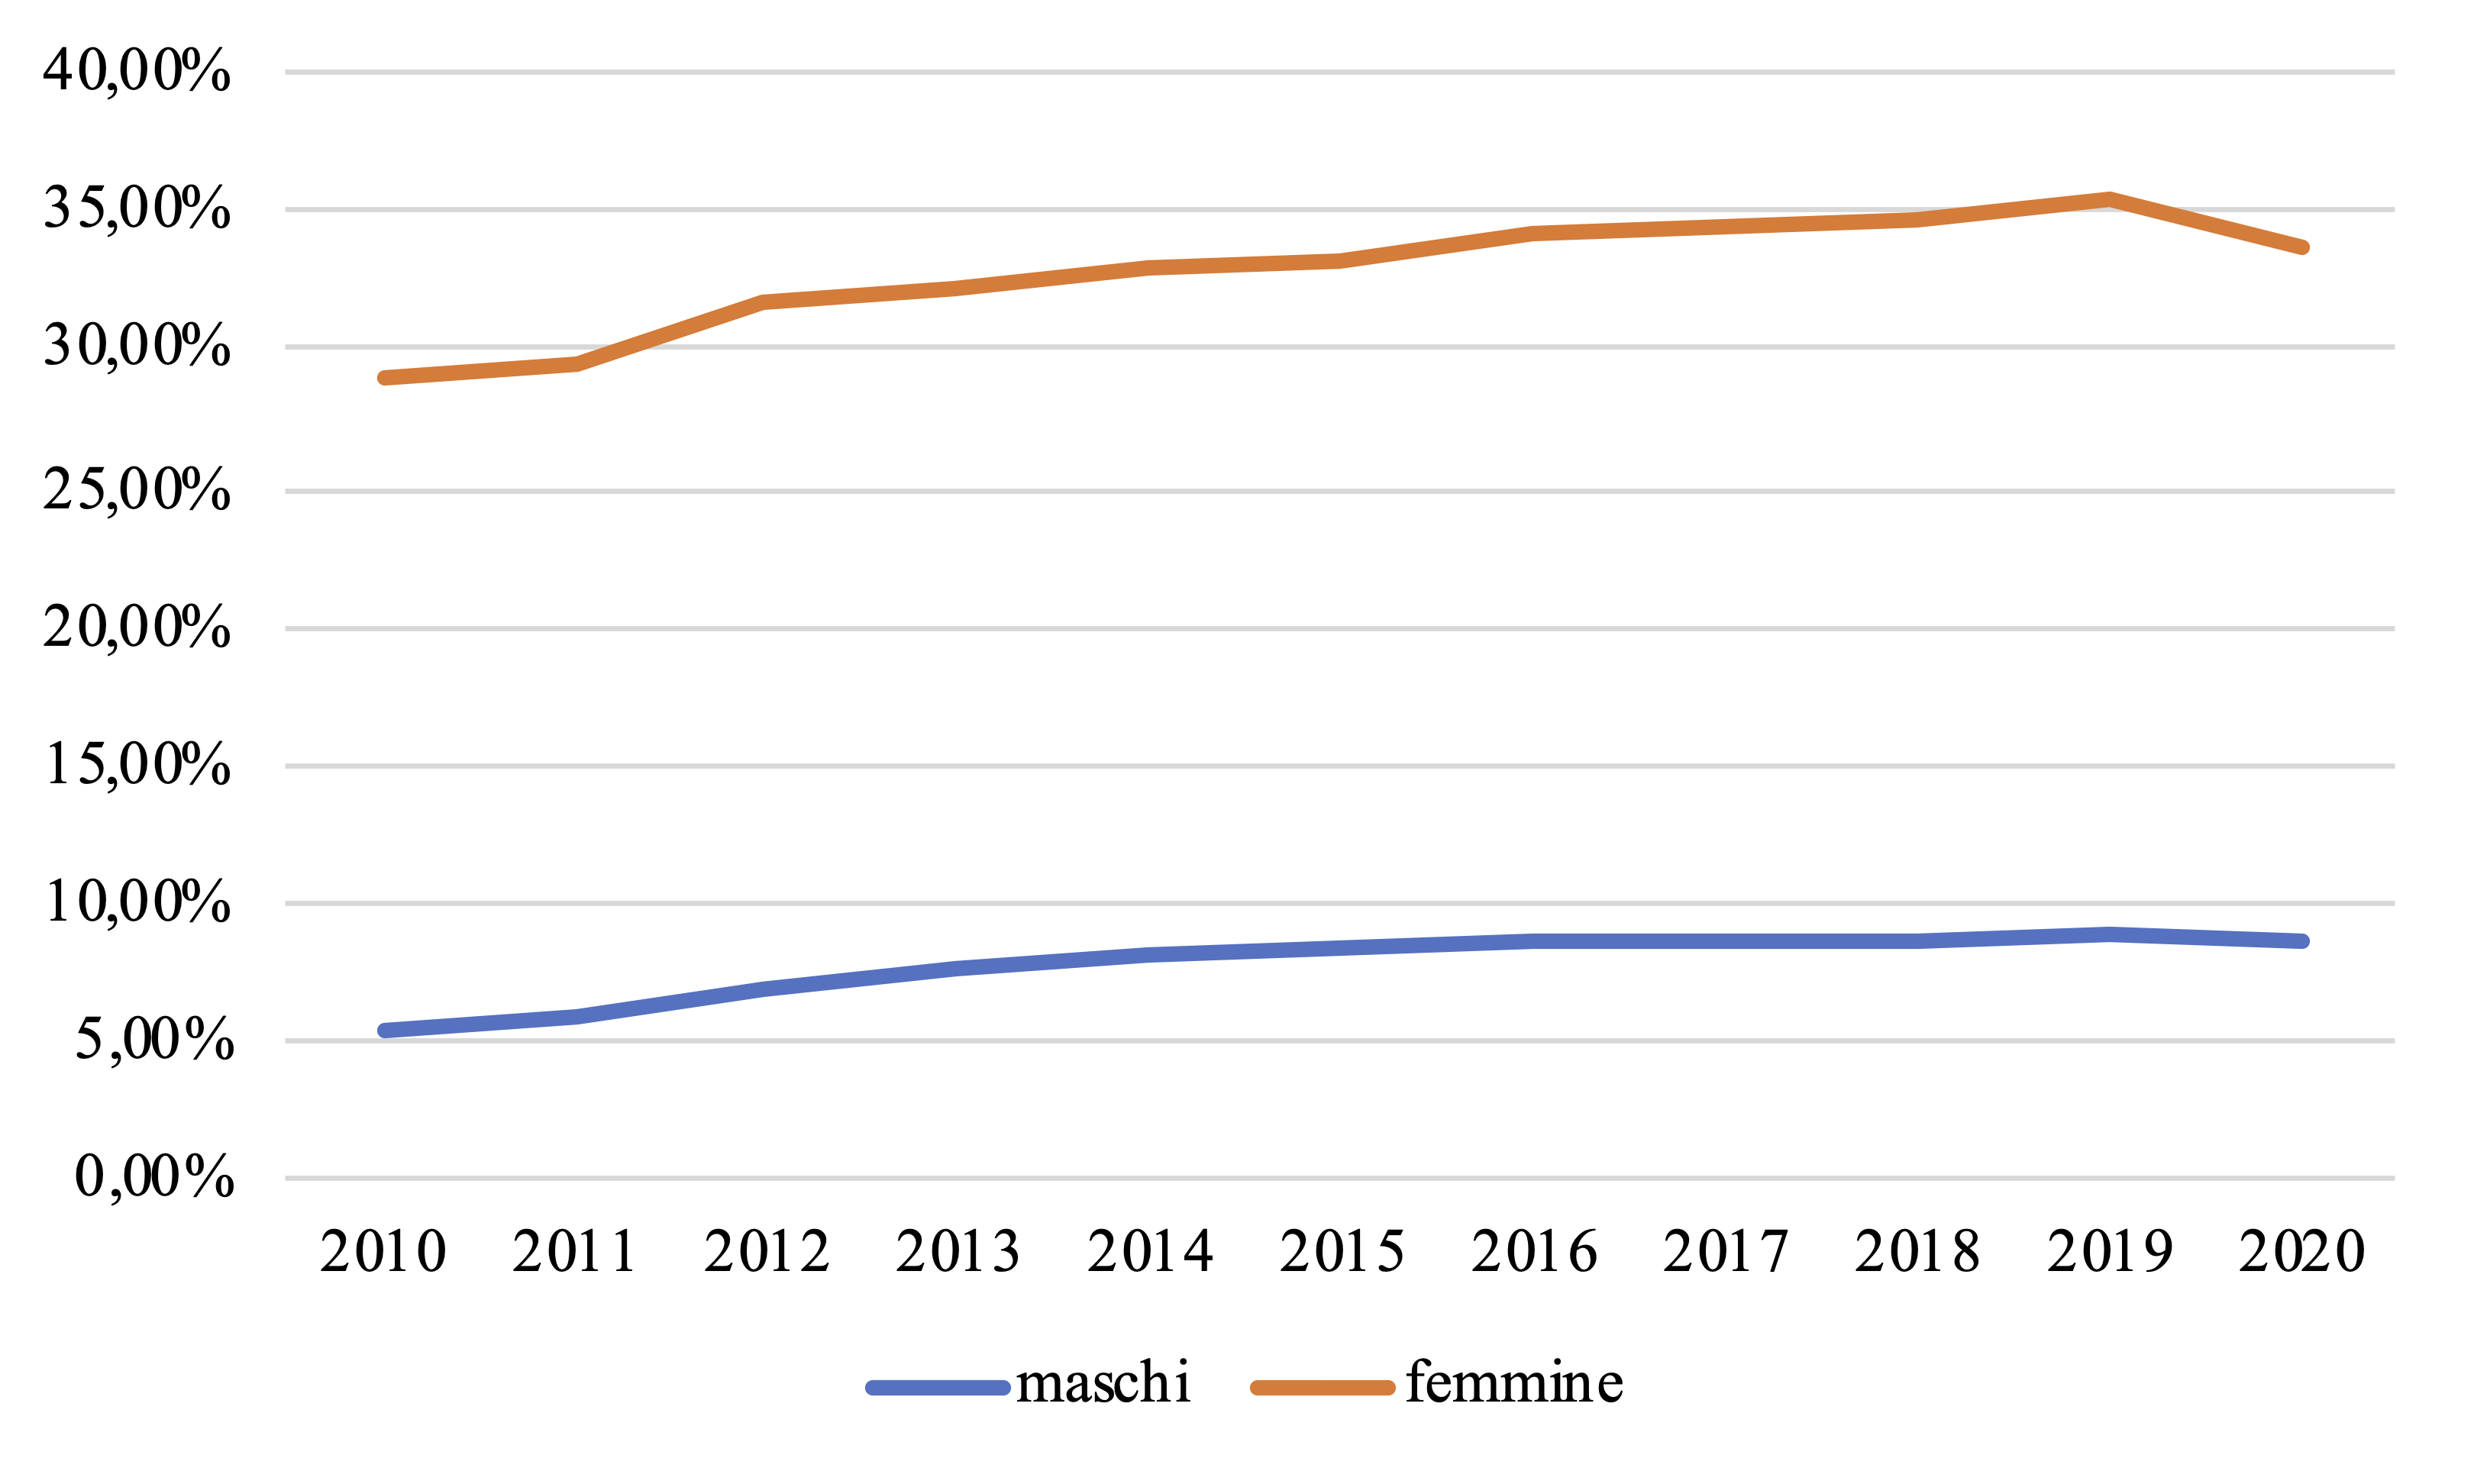
\includegraphics[width=\textwidth]{./images/part-time-rate-gender.png}
		\end{center}
			\caption{Part time rate}
	\end{minipage}
	\begin{minipage}[b]{0.5\textwidth}
		\begin{center}
			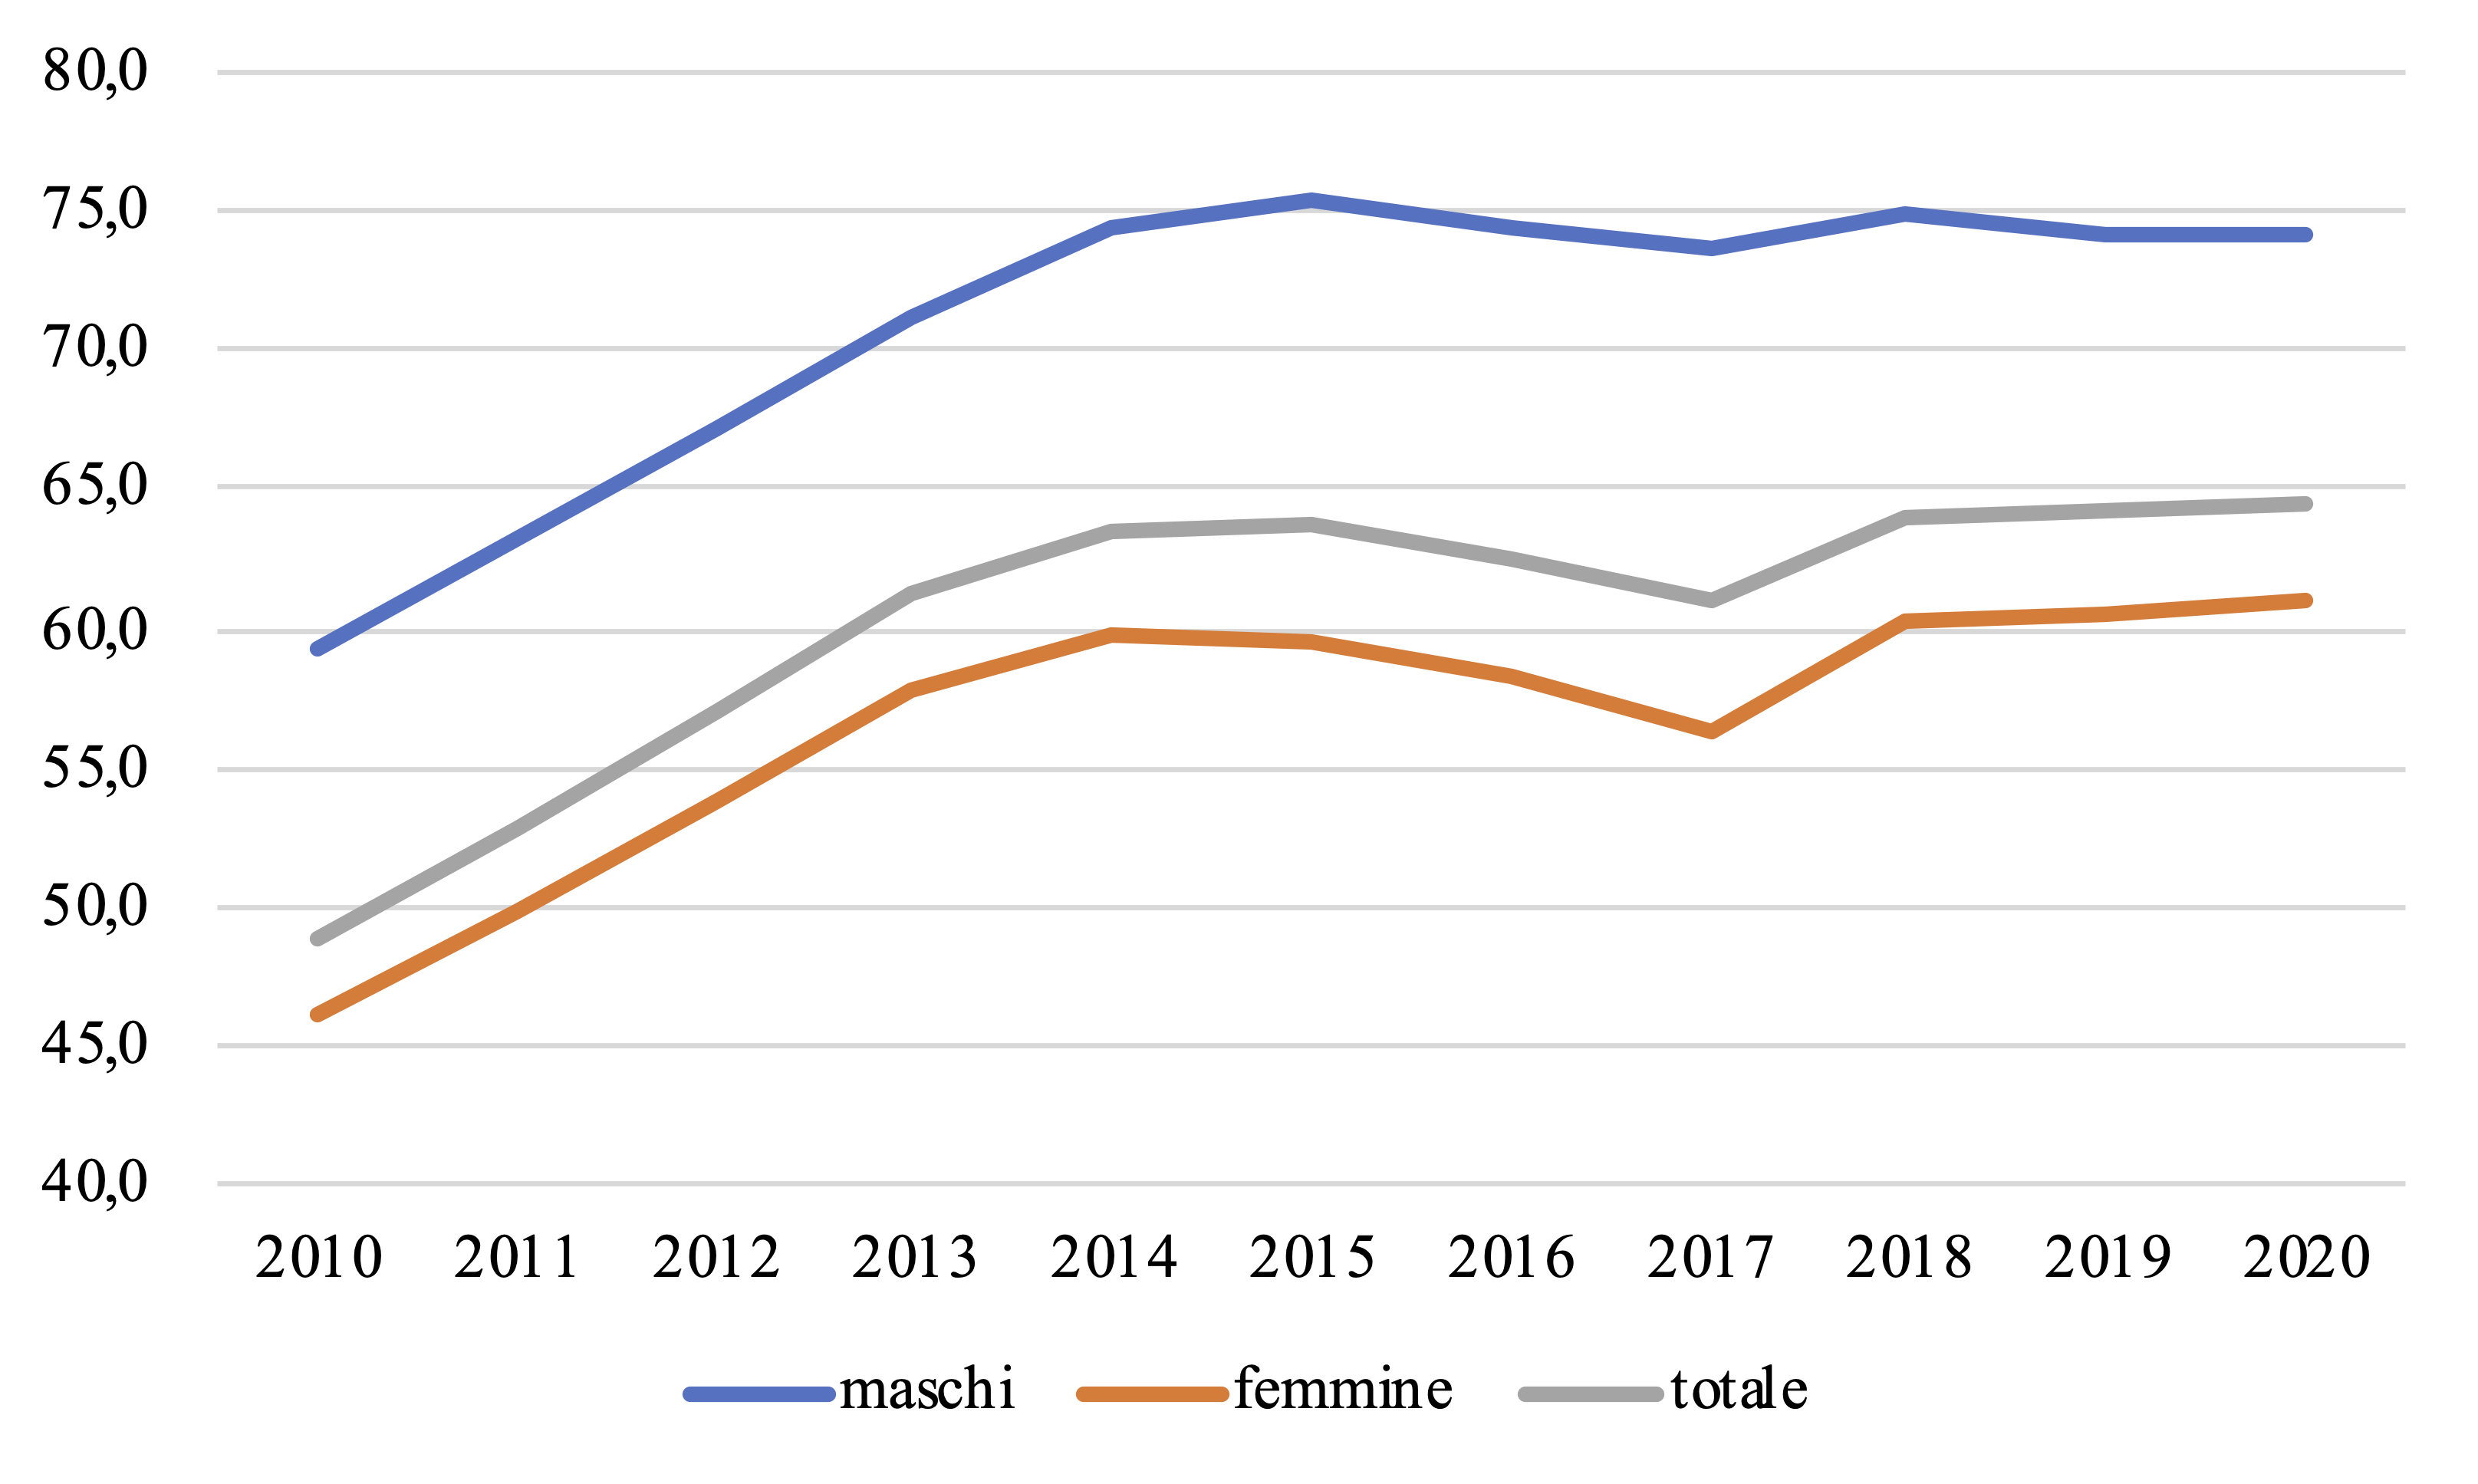
\includegraphics[width=\textwidth]{./images/prefer-part-time-gender.png}
		\end{center}
			\caption{Rate of preference of full time jobs by part time workers}
	\end{minipage}
\end{figure}

The median of weekly hours worked for men in 2020 was 38 while the same figure for women was 32. This was a small decrease from the 2019 value for men which was 40. Over time this values have remained relatively constant, 40 and 33 hours in 2010 for men and women. This may be related to the fact that the time women spend working at home doing jobs for which they are not financially compensated was 5 hours and 9 minutes in 2014 and 2 hours and 18 minutes for men. The time spent doing these jobs at home has increased for men and decreased for women since 2002. In 2002 the values were 1 hour and 59 minutes doing domestic work for men and 5 hours and 31 minutes for women. \cite{cappadozzi2019tempi}. Also, women are able to find a better work live balance even when measured with respect to work time \cite{canal2018punto}. These values remain constant over time.

Women are also affected in crisis but in a different way than men are. Women sometimes are obligated to remain active in the workforce while at the same time they perform care work. Moreover, in 2021, 35,663 women had to quit their jobs because they weren't able to balance professional care work. Of these 35,663, 35.3\% quit because the reasons they weren't able to balance work and care work were related to the company for which they worked for. In 2021 there were women 2,972 that requested more flexible work ours or to start working part time before they quit, only 1,673 had their requests granted. For men the number of requests was 137 and the number of requests granted was 73 \cite{del2022relazione}. There are also difficulties for women coming back from maternity leave and during pregnancy. Employers may exploit pregnant employees or impose unbearable conditions to keep the from coming back from maternity leave so that they quit their jobs. Other methods include refusal of transfer and refusal of permissions which these women are entitled to \cite{toffanin2018donne}.

\end{spacing}

\subsection{Region}

\begin{spacing}{1.5}

For a long time there has been a clear difference between the GDP of the different parts of Italy. More specifically, the differences between the North, Center and Mezzogiorno. It is important to understand the differences between these three in the short and long term to be able to make conclusions related to the income of people who live in these different regions. We can divide the differences between the North and Center against the Mezzogiorno into two categories. First are the geographical differences and second is the human element. We will see that the differences in the human element are long standing and have affected the Mezzogiorno for a long time.

In terms of natural endowments, southern Italy is a little disadvantaged but in a position comparable to that of central Italy. The differences are more pronounced within the macro areas than between them. This means that inside the north or south there will be places that are heavily disadvantaged in terms of geographic endowments like lack of access to water, fertile land or being located in terrain that is hard to access like mountains but there may also be places that are located in plains with fertile lands and easy access to water. An argument can be made that the north is located closer to the economic center of Europe. This may not have been true in the liberal age because of sea transportation. After the second world war, the difference had increased with the construction of highways that connected the North with the rest of Europe, this may have benefited the South as well but to a lesser degree than the north. These differences may explain the initial differences between the North and the South but not their evolutions to the differences that we see today.

The biggest differences that we see between the Mezzogiorno and the rest of Italy are in human and social capital. Human capital includes literacy and enrolment rates \cite{felice2012regional}. Social capital includes imbalances in the level of trust in political institutions and social participation. There are also differences in the personal distribution of income \cite{felice2013perche}. These differences are important because in the long run, GDP per capita followed these indicators and not the other way around. This means that when social and human capital were low, GDP per capita remained low. This becomes more important because when human capital was a significant variable for growth from 1891-1951 and when social capital was the significant conditioning variable from 1971 onwards the Mezzogiorno was not endowed with them.

The lack of these important variables can be attributed to a result of the different institutional settings that were in place before unification and persisted after it. Institutions in the Kingdom of the Two Sicilies were extractive \cite{robinson2012nations} while the northern states were inclusive. The differences in social and human capital can be said to stem from this \cite{felice2013perche}. After unification the northern states evolved into efficient liberal democracies while in the Mezzogiorno power continued to be distributed through nepotism, personal loyalty, or even violence. Moreover, in the souther states organized crime influenced social and economic life. Organized crime's power was strengthened with the creation of the new unified state through a mutual relationship of power. Organized crime was never put down when the opportunities came during unification or with the creation of the Republic.

\begin{figure}
	\begin{minipage}[b]{0.5\textwidth}
		\begin{center}
			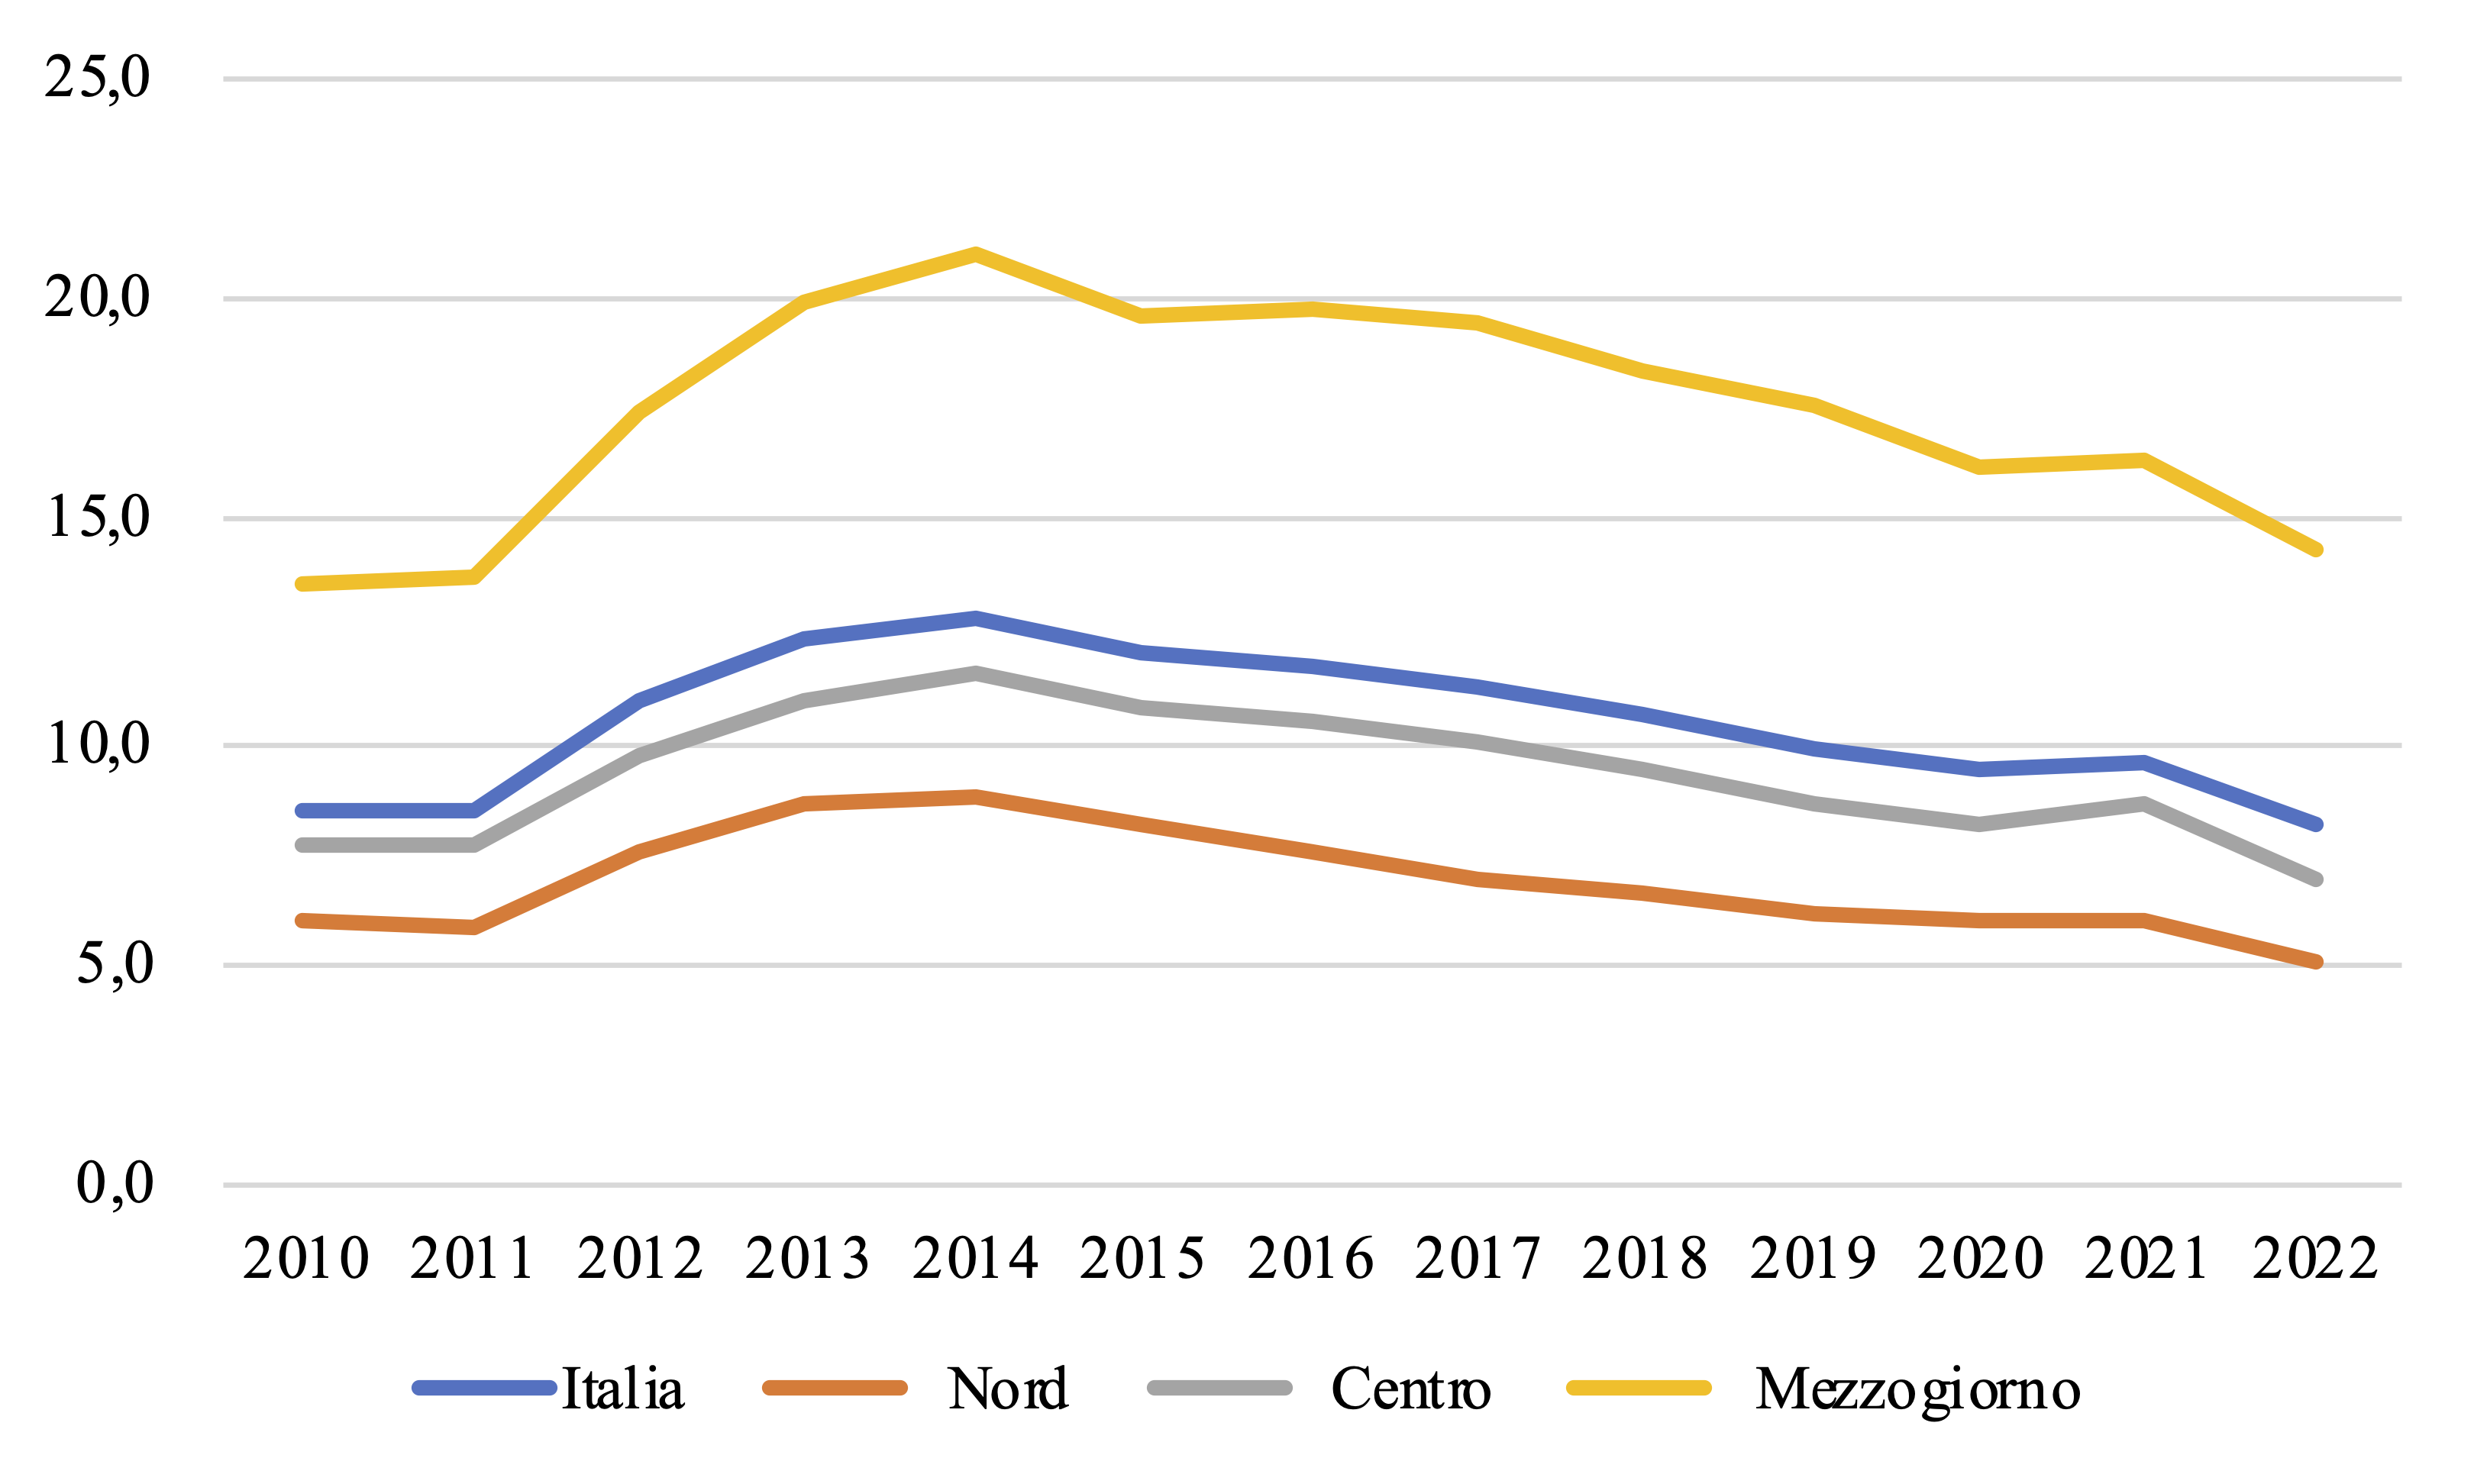
\includegraphics[width=\textwidth]{./images/unemployment-rate-regions.png}
		\end{center}
			\caption{Unemployment rate}
	\end{minipage}
	\begin{minipage}[b]{0.5\textwidth}
		\begin{center}
			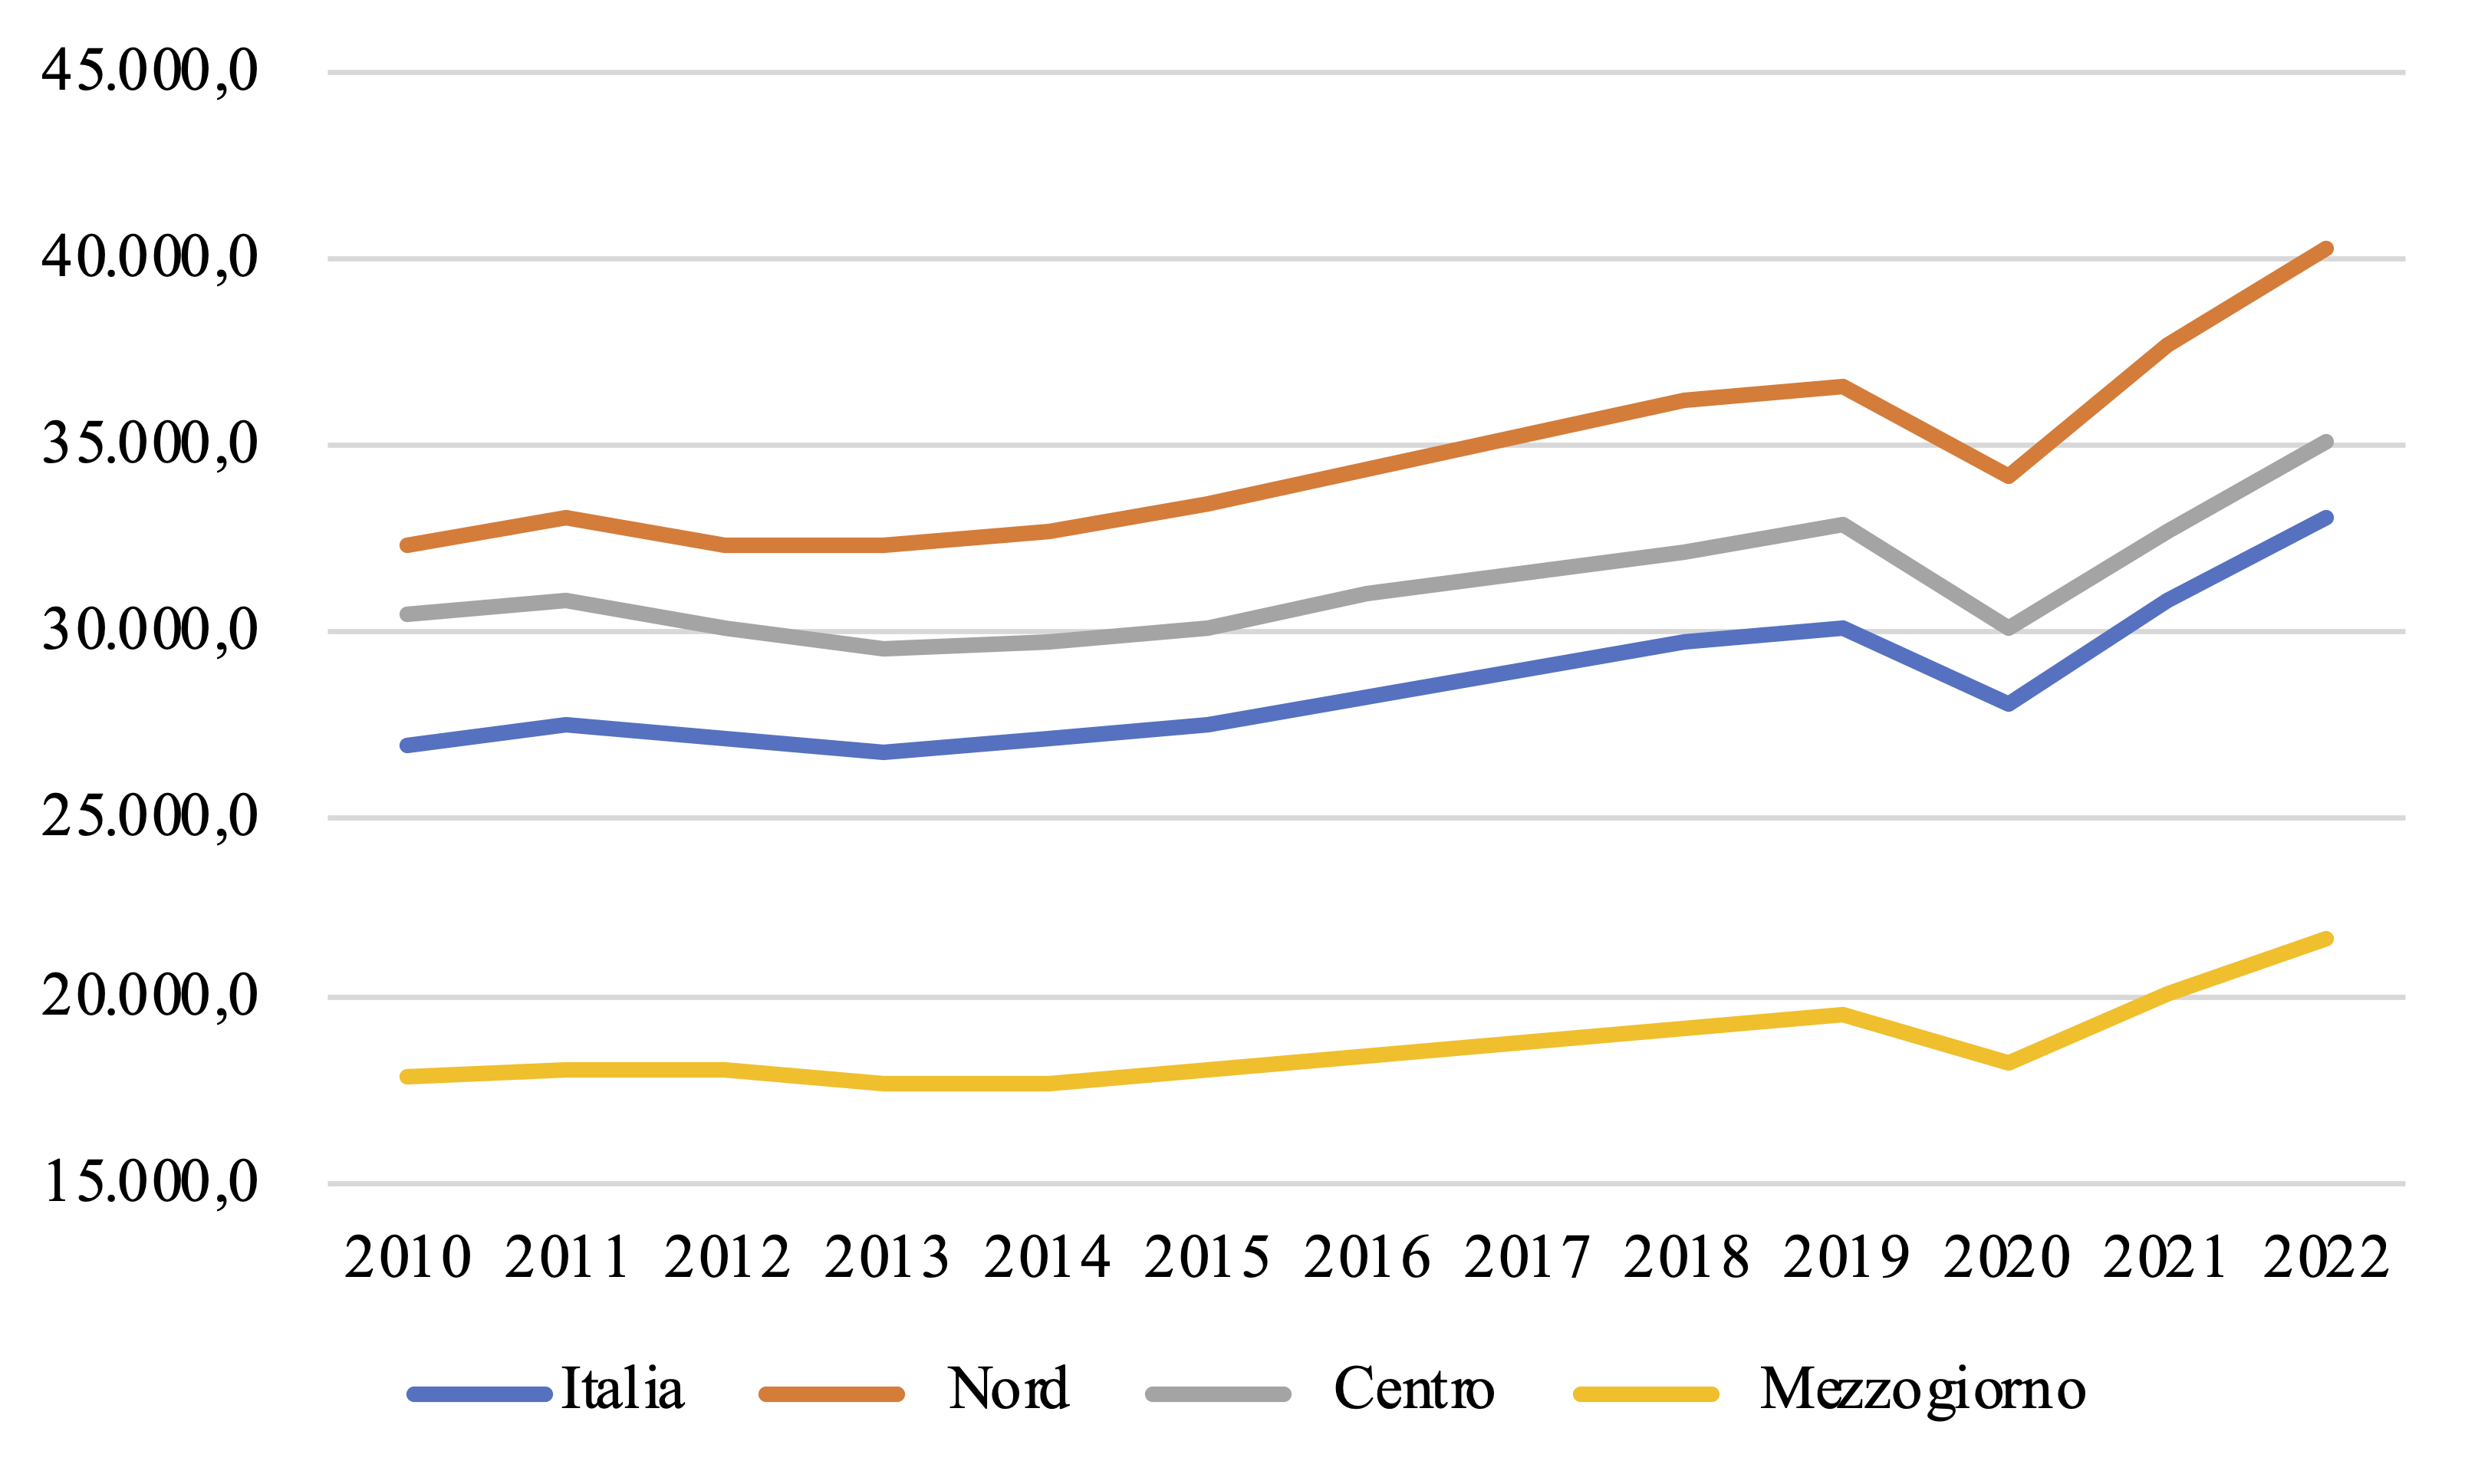
\includegraphics[width=\textwidth]{./images/gdp-per-capita-regions.png}
		\end{center}
			\caption{GDP per capita in euros}
	\end{minipage}
\end{figure}

The GDP per capita in the North for 2022 was 40,223, for the Center it was 35,051 and for the Mezzogiorno it was 21,653, the value for the Center-North was 32,983. There has been a significant increase to these values since 2010. There was a 24.84\% increase for the North, a 15.42\% increase for the Center, a 20.22\% increase in the Mezzogiorno and a 22.13\% increase in the Center-North. As we can see from this data, the Mezzogiorno still lags far behind the North and Center in terms of GDP per capita but we are starting to see a very gradual convergence of the Mezzogiorno and the Center if the current growth rates remain the same in the long run. The North still outpaces both the Center and Mezzogiorno. In terms of percent change between the years 2019 and 2020, the center north saw a greater contraction of their GDP per capita compared to the Mezzogiorno, a decrease of 7.38\% and a decrease of 6.33\% respectively. The province that saw the most growth since 2010 was Basilicata with an increase of 45.55\% and with a value of €27,751 in 2022 while the province with the least growth was Lazio with an increase 9.67\% and with a value of €37,180. In 2022 the unemployment rate in the North was 5.1\%, in the Center it was 7.0\%, and in the Mezzogiorno it was 14.3\%. Since 2010, the unemployment rate in the North has decreased by 0.9 percent points, in the Center by 0.7 and in the Mezzogiorno it has increased by 0.8 percent points. The rate of part time workers for the North in 2020 was 19.36\%, for the Center it was 20.08\% and for the Mezzogiorno it was 20.52\%. These values are similar but if we see the amount of growth since 2010 we can see the underlying differences. The unemployment rate in the North increased by 2.98 percent points from 2010 to 2020, in the Center the increase was of 3.11 percent points and in the Mezzogiorno there was an increase of 6.6\%

\end{spacing}

\section{Empirical Analysis}

\subsection{The Data}

\begin{spacing}{1.5}

The data used in this section will come from the Survey on Household Income and Wealth (SHIW) performed by the Banca d'Italia.  The SHIW was begun in the 1960s to gather data on the incomes and savings of Italian households. Over the years, the survey has grown in scope and now includes wealth and other aspects of households' economic and financial behaviour, including, for instance, the payment methods employed. The results of 2020, 2016, 2012, and 2008 will be used to see if there are any significant changes over time. The survey for the year 2020 was performed in the year 2021 due to the COVID-19 pandemic. 

%\begin{figure}
%	\caption{Datasets of the SHIW}
%\begin{center}
%	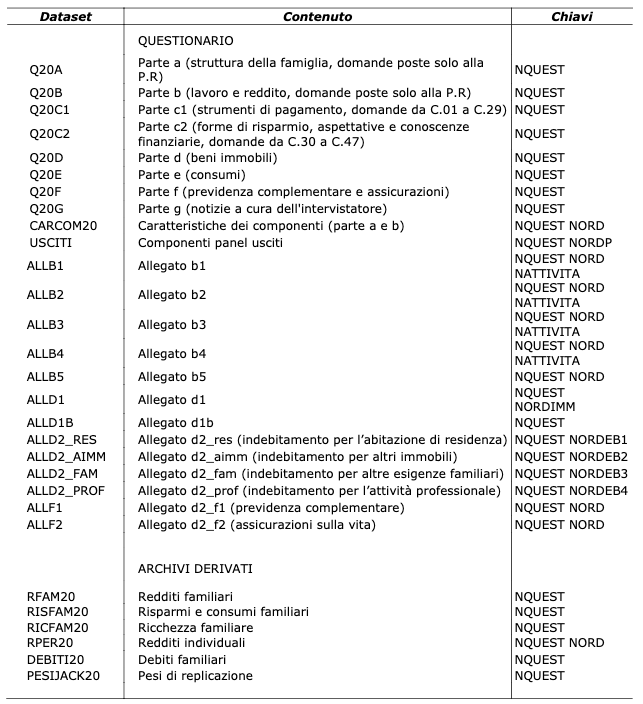
\includegraphics[width=14cm]{./images/datasets.png}
%\end{center}
%\end{figure}

I will be merging the datasets \verb+rfam(year).dta+ and \verb+carcom(year).dta+. The dataset \verb+rfam+ includes information on family income while the dataset \verb+carcom+ includes information on the participants of a specific family. This is done so that we can see the specific income of each family for all of the members of the family in question. The number of observations on each of these datasets are 15,198, 16,462, 20,022, and 19,907 for 2020, 2016, 2012, and 2008 respectively. These are the number of individuals.

\end{spacing}

\subsection{Methodology}

\begin{spacing}{1.5}

The model chosen was a multiple linear regression:

\begin{equation}
	y = {\beta}_{0} + {\beta}_{1} {x}_{1} + ... + {\beta}_{k} {x}_{k} + u
\end{equation}

This model allows us to control for many factors that affect the dependent variable, $ y $. This allows us to include more factors that may be related to our dependent variable thus allowing us to better explain its variation. Moreover, by controlling more factors, we are able to see better what is the specific effect of an independent variable on the dependent variable because we can hold the others fixed. The elements of the equation above can be explained as:

\begin{itemize}
	\item \textit{y}: this our dependant variable. The dependent variable will be family income.
	\item \textit{x}: are the regressors, the independent variables of our model.
	\item $ \beta $: these are the coefficients of our model.
	\item \textit{k}: this is the number of independent not including the intercept.
	\item \textit{u}: this is the error term, it accounts for all of the factors that affect \textit{y} but are not included in our model.
\end{itemize}

Furthermore, the model instead of using the absolute values of $ y $, we create a variable called $ ly $ which is the log of $ y $. This allows us to see the percentage effect that a change in $ x_i $ has on $ y $, allowing us to understand better the effects. Thus, our model can be expressed as:

\begin{equation}
	\mbox{log}(y) = {\widehat{\beta}}_{0} + {\widehat{\beta}}_{1} {x}_{1} + ... + {\widehat{\beta}}_{k} {x}_{k}
\end{equation}

where \textit{y} will be family income. There are hats over the $ \beta $s because these represent the sample coefficients. So, in this case, log(\textit{y}) is log(family income). The marginal effect of a change in $ {x}_{i} $ on $ y $ can be expressed as:

\begin{equation}
	\% \Delta y = ({\beta}_{i} 100) \Delta {x}_{i}
\end{equation}

The above is a percentage change in family income equals the change in $ x_i $ times the coefficient times 100. We multiply by 100 so that we get a percentage effect. Some of our independent variables will be dummy variables, they can either take the value 0 or 1, they take values 1 when they are true.Our independent variables of interest are:

\begin{itemize}
	\item \textbf{Gender}: we will see this variable represented in two different ways in our models, either we will use three dummy variables created for the model which are: Male and Married, Male and not Married, Female and Married. In this example the base group would be non married female. The other option is to include a single dummy variable called Male which is true if the observation is a man.
	\item \textbf{Age}: here we will also see age represented in two different ways. The first will be a group of dummy variables representing different age groups, the age groups are 0-34, 35-44, 45-54, 55-64, and over 64. In this case, the base group will be over 64. The other option is the use of two variables, the first is represents the age of the individual while the second is the age squared.
	\item \textbf{Region}: for region there will be only one option, there will be two dummy variables for North and Center and the base group will the Mezzogiorno.
\end{itemize}

Having two options for both Gender and Age will help us better understand the effects they have on log(family income).

\end{spacing}

\subsection{Age}

\begin{spacing}{1.5}

If we look at table \ref{table:age1}, we can see the model where age is represented as a group of different dummy variables. There are four dummy variables for four different age groups included in the model, 0-34, 35-44, 45-54, and 55-64. The base group in this model are ages over 64. Knowing this, we can see that the results of 2020 show that all of the age groups below over 64 have a lower family income. If an individual is 55-64 years old, his family income will be 10.79\% less than that of somebody who is over 64 holding other factors fixed. The results for the other groups are 25.49\%, 39.41\%, and 1.42\% for the 45-54, 35-44, and the 0-34 age groups respectively. The group that has the lowest family income across all four years is the 35-44 age group and it has been on a downward trend since at least 2008. There has been a 117.68\% decrease in this period of time. In fact, the numbers have been going down for all age groups except for the 0-34 age group. There has been a 265.71\% decreases for the 45-54 age group, and a 357.52\% decrease for the 55-64 age group. The value for the 0-34 age group in 2020 may be an anomaly due to its low significance level but if we perform an F-test including all four variables we can see that they together are significant enough to be included in the model, the result is a p-value of 0. Moreover, if we perform another F test to test if the result of the 0-34 age group is significantly different from that of the other age groups, the result is again a p-value of zero. Also, the decreasing trend that was being seen from 2008 to 2016 for the 0-34 age group was not very strong, so this may not be an anomaly.

\begin{table}[!h]
\caption{Model 2: Only Age Groups}
\centering
\begin{tabular}{lllllllll}
\cline{1-9}
\multicolumn{1}{r}{} &
  \multicolumn{2}{c}{ly} &
  \multicolumn{2}{c}{ly} &
  \multicolumn{2}{c}{ly} &
  \multicolumn{2}{c}{ly} \\
\cline{1-9}
\multicolumn{1}{l}{Less than 35} &
  \multicolumn{1}{r}{-0.1141} &
  \multicolumn{1}{l}{**} &
  \multicolumn{1}{r}{-0.1429} &
  \multicolumn{1}{l}{**} &
  \multicolumn{1}{r}{-0.1477} &
  \multicolumn{1}{l}{**} &
  \multicolumn{1}{r}{-0.0142} &
  \multicolumn{1}{l}{} \\
\multicolumn{1}{l}{35 to 44} &
  \multicolumn{1}{r}{-0.1810} &
  \multicolumn{1}{l}{**} &
  \multicolumn{1}{r}{-0.2928} &
  \multicolumn{1}{l}{**} &
  \multicolumn{1}{r}{-0.3433} &
  \multicolumn{1}{l}{**} &
  \multicolumn{1}{r}{-0.3941} &
  \multicolumn{1}{l}{**} \\
\multicolumn{1}{l}{45 to 54} &
  \multicolumn{1}{r}{-0.0697} &
  \multicolumn{1}{l}{**} &
  \multicolumn{1}{r}{-0.1408} &
  \multicolumn{1}{l}{**} &
  \multicolumn{1}{r}{-0.2783} &
  \multicolumn{1}{l}{**} &
  \multicolumn{1}{r}{-0.2549} &
  \multicolumn{1}{l}{**} \\
\multicolumn{1}{l}{55 to 64} &
  \multicolumn{1}{r}{0.0419} &
  \multicolumn{1}{l}{**} &
  \multicolumn{1}{r}{-0.0107} &
  \multicolumn{1}{l}{} &
  \multicolumn{1}{r}{-0.1212} &
  \multicolumn{1}{l}{**} &
  \multicolumn{1}{r}{-0.1079} &
  \multicolumn{1}{l}{**} \\
\multicolumn{1}{l}{Adjusted R-squared} &
  \multicolumn{1}{r}{0.44} &
  \multicolumn{1}{l}{} &
  \multicolumn{1}{r}{0.41} &
  \multicolumn{1}{l}{} &
  \multicolumn{1}{r}{0.38} &
  \multicolumn{1}{l}{} &
  \multicolumn{1}{r}{0.42} &
  \multicolumn{1}{l}{} \\
\cline{1-9}
\end{tabular}

\footnotesize{
** p$<$.01, * p$<$.05
}
\label{table:age1}
\end{table}

If we take a look at table \ref{table:age2} we can see the results of the third model where we have two variables for age. The first is age and the second is age squared. What this allows us to do it to see if there is a non linear relationship between age and family income. In our case, using this method is useful because we have very low p-values for all of the coefficients in all of the years, this shows us that both Age and Age Squared have a non null effect on log(family income). Furthermore, using these two variables, it allows us to see that first the relationship of age and family income is a negative one, as age increases, family income. Then, there is an inflexion point, from that point onward the relationship of age and income is positive, as age increases, income also increases. To find this inflexion point we need to use the following equation:

\begin{equation}
	\mbox{inflexion point} = abs \bigg(\frac{{\beta}_{age}}{2 {\beta}_{age^2}} \bigg)
\end{equation}

The results are 41 for 2008, 59 for 2012, 39.25 for 2016, and 43.83 for 2020. This means that according to the result for each year, from this age onwards age becomes a benefit rather than a detriment. From 2008 to 2020 this value has remained relatively stable.

\begin{table}[!h]
\caption{Model 3: Only Age}
\centering
\begin{tabular}{lllllllll}
\cline{1-9}
\multicolumn{1}{r}{} &
  \multicolumn{2}{c}{ly} &
  \multicolumn{2}{c}{ly} &
  \multicolumn{2}{c}{ly} &
  \multicolumn{2}{c}{ly} \\
\cline{1-9}
\multicolumn{1}{l}{Age} &
  \multicolumn{1}{r}{-0.0082} &
  \multicolumn{1}{l}{**} &
  \multicolumn{1}{r}{-0.0118} &
  \multicolumn{1}{l}{**} &
  \multicolumn{1}{r}{-0.0157} &
  \multicolumn{1}{l}{**} &
  \multicolumn{1}{r}{-0.0263} &
  \multicolumn{1}{l}{**} \\
\multicolumn{1}{l}{Age Squared} &
  \multicolumn{1}{r}{0.0001} &
  \multicolumn{1}{l}{**} &
  \multicolumn{1}{r}{0.0001} &
  \multicolumn{1}{l}{**} &
  \multicolumn{1}{r}{0.0002} &
  \multicolumn{1}{l}{**} &
  \multicolumn{1}{r}{0.0003} &
  \multicolumn{1}{l}{**} \\
\multicolumn{1}{l}{Adjusted R-squared} &
  \multicolumn{1}{r}{0.44} &
  \multicolumn{1}{l}{} &
  \multicolumn{1}{r}{0.41} &
  \multicolumn{1}{l}{} &
  \multicolumn{1}{r}{0.38} &
  \multicolumn{1}{l}{} &
  \multicolumn{1}{r}{0.42} &
  \multicolumn{1}{l}{} \\
\cline{1-9}
\end{tabular}

\footnotesize{
** p$<$.01, * p$<$.05
}
\label{table:age2}
\end{table}

\end{spacing}

\subsection{Gender}

\begin{spacing}{1.5}

If we look at table \ref{table:gender2} we can see that we have two dummy variables, one for Male and another for Married. We can see that in most years the coefficients are not statistically significant. But if we perform F-tests in which we include both Male and Married, for 2012, 2016, and 2020 the results are that the effects of Male and Married are significant with a p-value lower than 0.01 for all of these three years. This is not true for 2008 were the result of this same F-test results in a p-value of 0.1984. This is not an excellent result but it is good enough for them to still be included in the model. We can see from the table that either being male or female has a very small difference on family income. Compared to gender, the impact of marital status very large. A married person, regardless of gender, in 2020 has a family income 8.81\% greater than that of a non married person. Moreover, there seems to be a trend indicating a greater importance of being married, there has been an increase of 757.46\% to this coefficient since 2008.

\begin{table}[!h]
\caption{Model 2 - Only Gender and Marital Status}
\centering
\begin{tabular}{llllllll}
\cline{1-8}
\multicolumn{1}{r}{} &
  \multicolumn{1}{c}{ly} &
  \multicolumn{2}{c}{ly} &
  \multicolumn{2}{c}{ly} &
  \multicolumn{2}{c}{ly} \\
\cline{1-8}
\multicolumn{1}{l}{Male} &
  \multicolumn{1}{r}{0.0079} &
  \multicolumn{1}{r}{0.0175} &
  \multicolumn{1}{l}{*} &
  \multicolumn{1}{r}{0.0130} &
  \multicolumn{1}{l}{} &
  \multicolumn{1}{r}{-0.0014} &
  \multicolumn{1}{l}{} \\
\multicolumn{1}{l}{Married} &
  \multicolumn{1}{r}{-0.0134} &
  \multicolumn{1}{r}{0.0328} &
  \multicolumn{1}{l}{**} &
  \multicolumn{1}{r}{0.0992} &
  \multicolumn{1}{l}{**} &
  \multicolumn{1}{r}{0.0881} &
  \multicolumn{1}{l}{**} \\
\multicolumn{1}{l}{Adjusted R-squared} &
  \multicolumn{1}{r}{0.44} &
  \multicolumn{1}{r}{0.41} &
  \multicolumn{1}{l}{} &
  \multicolumn{1}{r}{0.38} &
  \multicolumn{1}{l}{} &
  \multicolumn{1}{r}{0.42} &
  \multicolumn{1}{l}{} \\
\cline{1-8}
\end{tabular}

\footnotesize{
** p$<$.01, * p$<$.05
}
\label{table:gender2}
\end{table}


\begin{table}[!h]
\caption{Model 1 - Only Gender and Marital Status}
\centering
\begin{tabular}{lllllllll}
\cline{1-9}
\multicolumn{1}{r}{} &
  \multicolumn{2}{c}{ly} &
  \multicolumn{2}{c}{ly} &
  \multicolumn{2}{c}{ly} &
  \multicolumn{2}{c}{ly} \\
\cline{1-9}
\multicolumn{1}{l}{Male and Married} &
  \multicolumn{1}{r}{-0.0116} &
  \multicolumn{1}{l}{} &
  \multicolumn{1}{r}{0.0430} &
  \multicolumn{1}{l}{**} &
  \multicolumn{1}{r}{0.1018} &
  \multicolumn{1}{l}{**} &
  \multicolumn{1}{r}{0.0823} &
  \multicolumn{1}{l}{**} \\
\multicolumn{1}{l}{Male and not Married} &
  \multicolumn{1}{r}{0.0519} &
  \multicolumn{1}{l}{**} &
  \multicolumn{1}{r}{0.0695} &
  \multicolumn{1}{l}{**} &
  \multicolumn{1}{r}{0.0719} &
  \multicolumn{1}{l}{**} &
  \multicolumn{1}{r}{0.0597} &
  \multicolumn{1}{l}{**} \\
\multicolumn{1}{l}{Female and Married} &
  \multicolumn{1}{r}{0.0226} &
  \multicolumn{1}{l}{*} &
  \multicolumn{1}{r}{0.0766} &
  \multicolumn{1}{l}{**} &
  \multicolumn{1}{r}{0.1505} &
  \multicolumn{1}{l}{**} &
  \multicolumn{1}{r}{0.1407} &
  \multicolumn{1}{l}{**} \\
\multicolumn{1}{l}{Adjusted R-squared} &
  \multicolumn{1}{r}{0.44} &
  \multicolumn{1}{l}{} &
  \multicolumn{1}{r}{0.42} &
  \multicolumn{1}{l}{} &
  \multicolumn{1}{r}{0.38} &
  \multicolumn{1}{l}{} &
  \multicolumn{1}{r}{0.42} &
  \multicolumn{1}{l}{} \\
\cline{1-9}
\end{tabular}

\footnotesize{
** p$<$.01, * p$<$.05
}
\label{table:gender1}
\end{table}

In the table \ref{table:gender1} we can see the model with three dummy variables. These variables are only true when both of the requirements are met. For example, Male and Married is equal to one only when the observation is both a man and he is married, it is not true for a man who is not married nor for a woman who is. Instantly we can see that the significance level of the variables included in this model are greater than the previous one, this is why there is this comparison between the two, it also allows us to better understand the effect of marital status and gender together. In this case the base group are women who are not married. We can see that any other of the three groups will have a greater family income than the base group. Observed men in general have a greater family income than women no matter the marital status. Also, married people have a greater family income no matter the gender. The group that has the greatest family income are married men who have a family income 8.23\% greater than unmarried women holding other factors fixed. In this model the importance of marital status has gone up over time as the coefficient of both Male and Married and Female and Married has gone up substantially since 2008. Moreover, the income for unmarried men has remained relatively constant since 2008. For 2008, an F-test was performed with the three dummy variables together to see whether they are statistically significant, the result is that they are with a p-value of 0.

\end{spacing}

\subsection{Region}

\begin{spacing}{1.5}

If we look at table \ref{table:reg1} we can see five dummy variables, two are for the region where the individual lives (North and Center) and the base group is the Mezzogiorno, the other five dummy variables correspond to the size of the municipality where the base group are mega municipalities, municipalities with a population greater than 500,000. We can see that if a person lives in the north in 2020, then his family income is 47.72\% greater than that of a person who lives in the Mezzogiorno holding other factors fixed. This value has increased over time from 35.8\% in 2008, this constitutes a 33.46\% increase. For the Center this value is 30.22\% in 2020 and has remained relatively stable over time.

In the table we can also see dummy variables for the size of the municipality where the person observed lives. Remembering that the base group is for municipalities with a population greater than 500,000, we can see that in most years a person who lives in a mega municipality has a greater family than a person who doesn't. This effect grows as the size of the municipality increases. This shows that there are intra region differences and not all municipalities of the North, Center or Mezzogiorno have the same family income just because they are in the same region. F-tests were conducted to see if the group of the size of municipalities is statistically significant to be included in the model for years 2008 and 2012, the results are that they are for both years with a p-value of 0.

\begin{table}[!ht]
\caption{Model 1 - Region and Municipality Size}
\centering
\begin{tabular}{lllllllll}
\cline{1-9}
\multicolumn{1}{r}{} &
  \multicolumn{2}{c}{ly} &
  \multicolumn{2}{c}{ly} &
  \multicolumn{2}{c}{ly} &
  \multicolumn{2}{c}{ly} \\
\cline{1-9}
\multicolumn{1}{l}{North} &
  \multicolumn{1}{r}{0.3580} &
  \multicolumn{1}{l}{**} &
  \multicolumn{1}{r}{0.3239} &
  \multicolumn{1}{l}{**} &
  \multicolumn{1}{r}{0.3218} &
  \multicolumn{1}{l}{**} &
  \multicolumn{1}{r}{0.4772} &
  \multicolumn{1}{l}{**} \\
\multicolumn{1}{l}{Center} &
  \multicolumn{1}{r}{0.3170} &
  \multicolumn{1}{l}{**} &
  \multicolumn{1}{r}{0.2785} &
  \multicolumn{1}{l}{**} &
  \multicolumn{1}{r}{0.2955} &
  \multicolumn{1}{l}{**} &
  \multicolumn{1}{r}{0.3022} &
  \multicolumn{1}{l}{**} \\
\multicolumn{1}{l}{Small Municipality} &
  \multicolumn{1}{r}{-0.0859} &
  \multicolumn{1}{l}{**} &
  \multicolumn{1}{r}{-0.0442} &
  \multicolumn{1}{l}{**} &
  \multicolumn{1}{r}{-0.1458} &
  \multicolumn{1}{l}{**} &
  \multicolumn{1}{r}{-0.4254} &
  \multicolumn{1}{l}{**} \\
\multicolumn{1}{l}{Medium Municipality} &
  \multicolumn{1}{r}{-0.0012} &
  \multicolumn{1}{l}{} &
  \multicolumn{1}{r}{-0.0122} &
  \multicolumn{1}{l}{} &
  \multicolumn{1}{r}{-0.0772} &
  \multicolumn{1}{l}{**} &
  \multicolumn{1}{r}{-0.2815} &
  \multicolumn{1}{l}{**} \\
\multicolumn{1}{l}{Large Municipality} &
  \multicolumn{1}{r}{-0.0198} &
  \multicolumn{1}{l}{} &
  \multicolumn{1}{r}{0.0011} &
  \multicolumn{1}{l}{} &
  \multicolumn{1}{r}{-0.1019} &
  \multicolumn{1}{l}{**} &
  \multicolumn{1}{r}{-0.2176} &
  \multicolumn{1}{l}{**} \\
\multicolumn{1}{l}{Adjusted R-squared} &
  \multicolumn{1}{r}{0.44} &
  \multicolumn{1}{l}{} &
  \multicolumn{1}{r}{0.42} &
  \multicolumn{1}{l}{} &
  \multicolumn{1}{r}{0.38} &
  \multicolumn{1}{l}{} &
  \multicolumn{1}{r}{0.42} &
  \multicolumn{1}{l}{} \\
\cline{1-9}
\end{tabular}

\footnotesize{
** p$<$.01, * p$<$.05
}
\label{table:reg1}
\end{table}

\end{spacing}

\subsection{Results}

\begin{table}[!h]
\caption{Model 1: Gender and Marital Status and Dummy Variables for Age Groups}
\centering
\begin{tabular}{lllllllll}
\cline{1-9}
\multicolumn{1}{r}{} &
  \multicolumn{2}{c}{ly} &
  \multicolumn{2}{c}{ly} &
  \multicolumn{2}{c}{ly} &
  \multicolumn{2}{c}{ly} \\
\cline{1-9}
\multicolumn{1}{l}{Male and Married} &
  \multicolumn{1}{r}{-0.0116} &
  \multicolumn{1}{l}{} &
  \multicolumn{1}{r}{0.0430} &
  \multicolumn{1}{l}{**} &
  \multicolumn{1}{r}{0.1018} &
  \multicolumn{1}{l}{**} &
  \multicolumn{1}{r}{0.0823} &
  \multicolumn{1}{l}{**} \\
\multicolumn{1}{l}{Male and not Married} &
  \multicolumn{1}{r}{0.0519} &
  \multicolumn{1}{l}{**} &
  \multicolumn{1}{r}{0.0695} &
  \multicolumn{1}{l}{**} &
  \multicolumn{1}{r}{0.0719} &
  \multicolumn{1}{l}{**} &
  \multicolumn{1}{r}{0.0597} &
  \multicolumn{1}{l}{**} \\
\multicolumn{1}{l}{Female and Married} &
  \multicolumn{1}{r}{0.0226} &
  \multicolumn{1}{l}{*} &
  \multicolumn{1}{r}{0.0766} &
  \multicolumn{1}{l}{**} &
  \multicolumn{1}{r}{0.1505} &
  \multicolumn{1}{l}{**} &
  \multicolumn{1}{r}{0.1407} &
  \multicolumn{1}{l}{**} \\
\multicolumn{1}{l}{University Degree or Higher} &
  \multicolumn{1}{r}{0.5156} &
  \multicolumn{1}{l}{**} &
  \multicolumn{1}{r}{0.5673} &
  \multicolumn{1}{l}{**} &
  \multicolumn{1}{r}{0.5535} &
  \multicolumn{1}{l}{**} &
  \multicolumn{1}{r}{0.7231} &
  \multicolumn{1}{l}{**} \\
\multicolumn{1}{l}{High School Diploma} &
  \multicolumn{1}{r}{0.2481} &
  \multicolumn{1}{l}{**} &
  \multicolumn{1}{r}{0.2797} &
  \multicolumn{1}{l}{**} &
  \multicolumn{1}{r}{0.2627} &
  \multicolumn{1}{l}{**} &
  \multicolumn{1}{r}{0.2558} &
  \multicolumn{1}{l}{**} \\
\multicolumn{1}{l}{Less than 35} &
  \multicolumn{1}{r}{-0.1309} &
  \multicolumn{1}{l}{**} &
  \multicolumn{1}{r}{-0.1618} &
  \multicolumn{1}{l}{**} &
  \multicolumn{1}{r}{-0.1711} &
  \multicolumn{1}{l}{**} &
  \multicolumn{1}{r}{-0.0319} &
  \multicolumn{1}{l}{} \\
\multicolumn{1}{l}{35 to 44} &
  \multicolumn{1}{r}{-0.1971} &
  \multicolumn{1}{l}{**} &
  \multicolumn{1}{r}{-0.3123} &
  \multicolumn{1}{l}{**} &
  \multicolumn{1}{r}{-0.3671} &
  \multicolumn{1}{l}{**} &
  \multicolumn{1}{r}{-0.4134} &
  \multicolumn{1}{l}{**} \\
\multicolumn{1}{l}{45 to 54} &
  \multicolumn{1}{r}{-0.0825} &
  \multicolumn{1}{l}{**} &
  \multicolumn{1}{r}{-0.1566} &
  \multicolumn{1}{l}{**} &
  \multicolumn{1}{r}{-0.2991} &
  \multicolumn{1}{l}{**} &
  \multicolumn{1}{r}{-0.2723} &
  \multicolumn{1}{l}{**} \\
\multicolumn{1}{l}{55 to 64} &
  \multicolumn{1}{r}{0.0350} &
  \multicolumn{1}{l}{**} &
  \multicolumn{1}{r}{-0.0199} &
  \multicolumn{1}{l}{} &
  \multicolumn{1}{r}{-0.1351} &
  \multicolumn{1}{l}{**} &
  \multicolumn{1}{r}{-0.1198} &
  \multicolumn{1}{l}{**} \\
\multicolumn{1}{l}{Family Members} &
  \multicolumn{1}{r}{0.3953} &
  \multicolumn{1}{l}{**} &
  \multicolumn{1}{r}{0.3013} &
  \multicolumn{1}{l}{**} &
  \multicolumn{1}{r}{0.2579} &
  \multicolumn{1}{l}{**} &
  \multicolumn{1}{r}{0.3555} &
  \multicolumn{1}{l}{**} \\
\multicolumn{1}{l}{Family Members Squared} &
  \multicolumn{1}{r}{-0.0450} &
  \multicolumn{1}{l}{**} &
  \multicolumn{1}{r}{-0.0340} &
  \multicolumn{1}{l}{**} &
  \multicolumn{1}{r}{-0.0283} &
  \multicolumn{1}{l}{**} &
  \multicolumn{1}{r}{-0.0385} &
  \multicolumn{1}{l}{**} \\
\multicolumn{1}{l}{Income Earners in Family} &
  \multicolumn{1}{r}{0.2811} &
  \multicolumn{1}{l}{**} &
  \multicolumn{1}{r}{0.3426} &
  \multicolumn{1}{l}{**} &
  \multicolumn{1}{r}{0.3426} &
  \multicolumn{1}{l}{**} &
  \multicolumn{1}{r}{0.3086} &
  \multicolumn{1}{l}{**} \\
\multicolumn{1}{l}{Autonomous Worker} &
  \multicolumn{1}{r}{0.1734} &
  \multicolumn{1}{l}{**} &
  \multicolumn{1}{r}{0.1331} &
  \multicolumn{1}{l}{**} &
  \multicolumn{1}{r}{0.1862} &
  \multicolumn{1}{l}{**} &
  \multicolumn{1}{r}{0.2836} &
  \multicolumn{1}{l}{**} \\
\multicolumn{1}{l}{Employee} &
  \multicolumn{1}{r}{0.0321} &
  \multicolumn{1}{l}{**} &
  \multicolumn{1}{r}{0.0308} &
  \multicolumn{1}{l}{**} &
  \multicolumn{1}{r}{0.1333} &
  \multicolumn{1}{l}{**} &
  \multicolumn{1}{r}{0.0257} &
  \multicolumn{1}{l}{} \\
\multicolumn{1}{l}{North} &
  \multicolumn{1}{r}{0.3580} &
  \multicolumn{1}{l}{**} &
  \multicolumn{1}{r}{0.3239} &
  \multicolumn{1}{l}{**} &
  \multicolumn{1}{r}{0.3218} &
  \multicolumn{1}{l}{**} &
  \multicolumn{1}{r}{0.4772} &
  \multicolumn{1}{l}{**} \\
\multicolumn{1}{l}{Center} &
  \multicolumn{1}{r}{0.3170} &
  \multicolumn{1}{l}{**} &
  \multicolumn{1}{r}{0.2785} &
  \multicolumn{1}{l}{**} &
  \multicolumn{1}{r}{0.2955} &
  \multicolumn{1}{l}{**} &
  \multicolumn{1}{r}{0.3022} &
  \multicolumn{1}{l}{**} \\
\multicolumn{1}{l}{Small Municipality} &
  \multicolumn{1}{r}{-0.0859} &
  \multicolumn{1}{l}{**} &
  \multicolumn{1}{r}{-0.0442} &
  \multicolumn{1}{l}{**} &
  \multicolumn{1}{r}{-0.1458} &
  \multicolumn{1}{l}{**} &
  \multicolumn{1}{r}{-0.4254} &
  \multicolumn{1}{l}{**} \\
\multicolumn{1}{l}{Medium Municipality} &
  \multicolumn{1}{r}{-0.0012} &
  \multicolumn{1}{l}{} &
  \multicolumn{1}{r}{-0.0122} &
  \multicolumn{1}{l}{} &
  \multicolumn{1}{r}{-0.0772} &
  \multicolumn{1}{l}{**} &
  \multicolumn{1}{r}{-0.2815} &
  \multicolumn{1}{l}{**} \\
\multicolumn{1}{l}{Large Municipality} &
  \multicolumn{1}{r}{-0.0198} &
  \multicolumn{1}{l}{} &
  \multicolumn{1}{r}{0.0011} &
  \multicolumn{1}{l}{} &
  \multicolumn{1}{r}{-0.1019} &
  \multicolumn{1}{l}{**} &
  \multicolumn{1}{r}{-0.2176} &
  \multicolumn{1}{l}{**} \\
\multicolumn{1}{l}{Intercept} &
  \multicolumn{1}{r}{8.7996} &
  \multicolumn{1}{l}{**} &
  \multicolumn{1}{r}{8.8322} &
  \multicolumn{1}{l}{**} &
  \multicolumn{1}{r}{8.9674} &
  \multicolumn{1}{l}{**} &
  \multicolumn{1}{r}{9.1280} &
  \multicolumn{1}{l}{**} \\
\multicolumn{1}{l}{Adjusted R-squared} &
  \multicolumn{1}{r}{0.44} &
  \multicolumn{1}{l}{} &
  \multicolumn{1}{r}{0.42} &
  \multicolumn{1}{l}{} &
  \multicolumn{1}{r}{0.38} &
  \multicolumn{1}{l}{} &
  \multicolumn{1}{r}{0.42} &
  \multicolumn{1}{l}{} \\
\cline{1-9}
\end{tabular}

\footnotesize{
** p$<$.01, * p$<$.05
}
\end{table}

\clearpage

\begin{table}[!h]
\caption{Model 2: Single Dummy Variable for Gender and Dummy Variables for Age Groups}
\centering
\begin{tabular}{lllllllll}
\cline{1-9}
\multicolumn{1}{r}{} &
  \multicolumn{2}{c}{ly} &
  \multicolumn{2}{c}{ly} &
  \multicolumn{2}{c}{ly} &
  \multicolumn{2}{c}{ly} \\
\cline{1-9}
\multicolumn{1}{l}{Male} &
  \multicolumn{1}{r}{0.0079} &
  \multicolumn{1}{l}{} &
  \multicolumn{1}{r}{0.0175} &
  \multicolumn{1}{l}{*} &
  \multicolumn{1}{r}{0.0130} &
  \multicolumn{1}{l}{} &
  \multicolumn{1}{r}{-0.0014} &
  \multicolumn{1}{l}{} \\
\multicolumn{1}{l}{Married} &
  \multicolumn{1}{r}{-0.0134} &
  \multicolumn{1}{l}{} &
  \multicolumn{1}{r}{0.0328} &
  \multicolumn{1}{l}{**} &
  \multicolumn{1}{r}{0.0992} &
  \multicolumn{1}{l}{**} &
  \multicolumn{1}{r}{0.0881} &
  \multicolumn{1}{l}{**} \\
\multicolumn{1}{l}{University Degree or Higher} &
  \multicolumn{1}{r}{0.5161} &
  \multicolumn{1}{l}{**} &
  \multicolumn{1}{r}{0.5676} &
  \multicolumn{1}{l}{**} &
  \multicolumn{1}{r}{0.5538} &
  \multicolumn{1}{l}{**} &
  \multicolumn{1}{r}{0.7246} &
  \multicolumn{1}{l}{**} \\
\multicolumn{1}{l}{High School Diploma} &
  \multicolumn{1}{r}{0.2485} &
  \multicolumn{1}{l}{**} &
  \multicolumn{1}{r}{0.2807} &
  \multicolumn{1}{l}{**} &
  \multicolumn{1}{r}{0.2639} &
  \multicolumn{1}{l}{**} &
  \multicolumn{1}{r}{0.2573} &
  \multicolumn{1}{l}{**} \\
\multicolumn{1}{l}{Less than 35} &
  \multicolumn{1}{r}{-0.1141} &
  \multicolumn{1}{l}{**} &
  \multicolumn{1}{r}{-0.1429} &
  \multicolumn{1}{l}{**} &
  \multicolumn{1}{r}{-0.1477} &
  \multicolumn{1}{l}{**} &
  \multicolumn{1}{r}{-0.0142} &
  \multicolumn{1}{l}{} \\
\multicolumn{1}{l}{35 to 44} &
  \multicolumn{1}{r}{-0.1810} &
  \multicolumn{1}{l}{**} &
  \multicolumn{1}{r}{-0.2928} &
  \multicolumn{1}{l}{**} &
  \multicolumn{1}{r}{-0.3433} &
  \multicolumn{1}{l}{**} &
  \multicolumn{1}{r}{-0.3941} &
  \multicolumn{1}{l}{**} \\
\multicolumn{1}{l}{45 to 54} &
  \multicolumn{1}{r}{-0.0697} &
  \multicolumn{1}{l}{**} &
  \multicolumn{1}{r}{-0.1408} &
  \multicolumn{1}{l}{**} &
  \multicolumn{1}{r}{-0.2783} &
  \multicolumn{1}{l}{**} &
  \multicolumn{1}{r}{-0.2549} &
  \multicolumn{1}{l}{**} \\
\multicolumn{1}{l}{55 to 64} &
  \multicolumn{1}{r}{0.0419} &
  \multicolumn{1}{l}{**} &
  \multicolumn{1}{r}{-0.0107} &
  \multicolumn{1}{l}{} &
  \multicolumn{1}{r}{-0.1212} &
  \multicolumn{1}{l}{**} &
  \multicolumn{1}{r}{-0.1079} &
  \multicolumn{1}{l}{**} \\
\multicolumn{1}{l}{Family Members} &
  \multicolumn{1}{r}{0.3915} &
  \multicolumn{1}{l}{**} &
  \multicolumn{1}{r}{0.2976} &
  \multicolumn{1}{l}{**} &
  \multicolumn{1}{r}{0.2524} &
  \multicolumn{1}{l}{**} &
  \multicolumn{1}{r}{0.3482} &
  \multicolumn{1}{l}{**} \\
\multicolumn{1}{l}{Family Members Squared} &
  \multicolumn{1}{r}{-0.0447} &
  \multicolumn{1}{l}{**} &
  \multicolumn{1}{r}{-0.0337} &
  \multicolumn{1}{l}{**} &
  \multicolumn{1}{r}{-0.0279} &
  \multicolumn{1}{l}{**} &
  \multicolumn{1}{r}{-0.0379} &
  \multicolumn{1}{l}{**} \\
\multicolumn{1}{l}{Income Earners in Family} &
  \multicolumn{1}{r}{0.2839} &
  \multicolumn{1}{l}{**} &
  \multicolumn{1}{r}{0.3460} &
  \multicolumn{1}{l}{**} &
  \multicolumn{1}{r}{0.3468} &
  \multicolumn{1}{l}{**} &
  \multicolumn{1}{r}{0.3120} &
  \multicolumn{1}{l}{**} \\
\multicolumn{1}{l}{Autonomous Worker} &
  \multicolumn{1}{r}{0.1633} &
  \multicolumn{1}{l}{**} &
  \multicolumn{1}{r}{0.1209} &
  \multicolumn{1}{l}{**} &
  \multicolumn{1}{r}{0.1742} &
  \multicolumn{1}{l}{**} &
  \multicolumn{1}{r}{0.2714} &
  \multicolumn{1}{l}{**} \\
\multicolumn{1}{l}{Employee} &
  \multicolumn{1}{r}{0.0237} &
  \multicolumn{1}{l}{*} &
  \multicolumn{1}{r}{0.0200} &
  \multicolumn{1}{l}{} &
  \multicolumn{1}{r}{0.1213} &
  \multicolumn{1}{l}{**} &
  \multicolumn{1}{r}{0.0179} &
  \multicolumn{1}{l}{} \\
\multicolumn{1}{l}{North} &
  \multicolumn{1}{r}{0.3580} &
  \multicolumn{1}{l}{**} &
  \multicolumn{1}{r}{0.3242} &
  \multicolumn{1}{l}{**} &
  \multicolumn{1}{r}{0.3218} &
  \multicolumn{1}{l}{**} &
  \multicolumn{1}{r}{0.4775} &
  \multicolumn{1}{l}{**} \\
\multicolumn{1}{l}{Center} &
  \multicolumn{1}{r}{0.3170} &
  \multicolumn{1}{l}{**} &
  \multicolumn{1}{r}{0.2784} &
  \multicolumn{1}{l}{**} &
  \multicolumn{1}{r}{0.2955} &
  \multicolumn{1}{l}{**} &
  \multicolumn{1}{r}{0.3022} &
  \multicolumn{1}{l}{**} \\
\multicolumn{1}{l}{Small Municipality} &
  \multicolumn{1}{r}{-0.0863} &
  \multicolumn{1}{l}{**} &
  \multicolumn{1}{r}{-0.0442} &
  \multicolumn{1}{l}{**} &
  \multicolumn{1}{r}{-0.1455} &
  \multicolumn{1}{l}{**} &
  \multicolumn{1}{r}{-0.4253} &
  \multicolumn{1}{l}{**} \\
\multicolumn{1}{l}{Medium Municipality} &
  \multicolumn{1}{r}{-0.0014} &
  \multicolumn{1}{l}{} &
  \multicolumn{1}{r}{-0.0130} &
  \multicolumn{1}{l}{} &
  \multicolumn{1}{r}{-0.0784} &
  \multicolumn{1}{l}{**} &
  \multicolumn{1}{r}{-0.2813} &
  \multicolumn{1}{l}{**} \\
\multicolumn{1}{l}{Large Municipality} &
  \multicolumn{1}{r}{-0.0204} &
  \multicolumn{1}{l}{} &
  \multicolumn{1}{r}{0.0007} &
  \multicolumn{1}{l}{} &
  \multicolumn{1}{r}{-0.1023} &
  \multicolumn{1}{l}{**} &
  \multicolumn{1}{r}{-0.2178} &
  \multicolumn{1}{l}{**} \\
\multicolumn{1}{l}{Intercept} &
  \multicolumn{1}{r}{8.8130} &
  \multicolumn{1}{l}{**} &
  \multicolumn{1}{r}{8.8476} &
  \multicolumn{1}{l}{**} &
  \multicolumn{1}{r}{8.9860} &
  \multicolumn{1}{l}{**} &
  \multicolumn{1}{r}{9.1548} &
  \multicolumn{1}{l}{**} \\
\multicolumn{1}{l}{Adjusted R-squared} &
  \multicolumn{1}{r}{0.44} &
  \multicolumn{1}{l}{} &
  \multicolumn{1}{r}{0.41} &
  \multicolumn{1}{l}{} &
  \multicolumn{1}{r}{0.38} &
  \multicolumn{1}{l}{} &
  \multicolumn{1}{r}{0.42} &
  \multicolumn{1}{l}{} \\
\cline{1-9}
\end{tabular}

\footnotesize{
** p$<$.01, * p$<$.05
}
\end{table}

\begin{table}[!h]
\caption{Model 3: Single Dummy Variable for Gender and Age with Quadratic}
\centering
\begin{tabular}{lllllllll}
\cline{1-9}
\multicolumn{1}{r}{} &
  \multicolumn{2}{c}{ly} &
  \multicolumn{2}{c}{ly} &
  \multicolumn{2}{c}{ly} &
  \multicolumn{2}{c}{ly} \\
\cline{1-9}
\multicolumn{1}{l}{Male} &
  \multicolumn{1}{r}{0.0081} &
  \multicolumn{1}{l}{} &
  \multicolumn{1}{r}{0.0180} &
  \multicolumn{1}{l}{*} &
  \multicolumn{1}{r}{0.0185} &
  \multicolumn{1}{l}{} &
  \multicolumn{1}{r}{0.0007} &
  \multicolumn{1}{l}{} \\
\multicolumn{1}{l}{Married} &
  \multicolumn{1}{r}{0.0612} &
  \multicolumn{1}{l}{**} &
  \multicolumn{1}{r}{0.1092} &
  \multicolumn{1}{l}{**} &
  \multicolumn{1}{r}{0.1679} &
  \multicolumn{1}{l}{**} &
  \multicolumn{1}{r}{0.1600} &
  \multicolumn{1}{l}{**} \\
\multicolumn{1}{l}{University Degree or Higher} &
  \multicolumn{1}{r}{0.5303} &
  \multicolumn{1}{l}{**} &
  \multicolumn{1}{r}{0.5831} &
  \multicolumn{1}{l}{**} &
  \multicolumn{1}{r}{0.5780} &
  \multicolumn{1}{l}{**} &
  \multicolumn{1}{r}{0.7814} &
  \multicolumn{1}{l}{**} \\
\multicolumn{1}{l}{High School Diploma} &
  \multicolumn{1}{r}{0.2599} &
  \multicolumn{1}{l}{**} &
  \multicolumn{1}{r}{0.2990} &
  \multicolumn{1}{l}{**} &
  \multicolumn{1}{r}{0.2882} &
  \multicolumn{1}{l}{**} &
  \multicolumn{1}{r}{0.3169} &
  \multicolumn{1}{l}{**} \\
\multicolumn{1}{l}{Age} &
  \multicolumn{1}{r}{-0.0082} &
  \multicolumn{1}{l}{**} &
  \multicolumn{1}{r}{-0.0118} &
  \multicolumn{1}{l}{**} &
  \multicolumn{1}{r}{-0.0157} &
  \multicolumn{1}{l}{**} &
  \multicolumn{1}{r}{-0.0263} &
  \multicolumn{1}{l}{**} \\
\multicolumn{1}{l}{Age Squared} &
  \multicolumn{1}{r}{0.0001} &
  \multicolumn{1}{l}{**} &
  \multicolumn{1}{r}{0.0001} &
  \multicolumn{1}{l}{**} &
  \multicolumn{1}{r}{0.0002} &
  \multicolumn{1}{l}{**} &
  \multicolumn{1}{r}{0.0003} &
  \multicolumn{1}{l}{**} \\
\multicolumn{1}{l}{Family Members} &
  \multicolumn{1}{r}{0.3419} &
  \multicolumn{1}{l}{**} &
  \multicolumn{1}{r}{0.2475} &
  \multicolumn{1}{l}{**} &
  \multicolumn{1}{r}{0.1922} &
  \multicolumn{1}{l}{**} &
  \multicolumn{1}{r}{0.2802} &
  \multicolumn{1}{l}{**} \\
\multicolumn{1}{l}{Family Members Squared} &
  \multicolumn{1}{r}{-0.0406} &
  \multicolumn{1}{l}{**} &
  \multicolumn{1}{r}{-0.0299} &
  \multicolumn{1}{l}{**} &
  \multicolumn{1}{r}{-0.0235} &
  \multicolumn{1}{l}{**} &
  \multicolumn{1}{r}{-0.0325} &
  \multicolumn{1}{l}{**} \\
\multicolumn{1}{l}{Income Earners in Family} &
  \multicolumn{1}{r}{0.3024} &
  \multicolumn{1}{l}{**} &
  \multicolumn{1}{r}{0.3651} &
  \multicolumn{1}{l}{**} &
  \multicolumn{1}{r}{0.3721} &
  \multicolumn{1}{l}{**} &
  \multicolumn{1}{r}{0.3372} &
  \multicolumn{1}{l}{**} \\
\multicolumn{1}{l}{Autonomous Worker} &
  \multicolumn{1}{r}{0.1662} &
  \multicolumn{1}{l}{**} &
  \multicolumn{1}{r}{0.1190} &
  \multicolumn{1}{l}{**} &
  \multicolumn{1}{r}{0.1430} &
  \multicolumn{1}{l}{**} &
  \multicolumn{1}{r}{0.2685} &
  \multicolumn{1}{l}{**} \\
\multicolumn{1}{l}{Employee} &
  \multicolumn{1}{r}{0.0180} &
  \multicolumn{1}{l}{} &
  \multicolumn{1}{r}{0.0095} &
  \multicolumn{1}{l}{} &
  \multicolumn{1}{r}{0.0812} &
  \multicolumn{1}{l}{**} &
  \multicolumn{1}{r}{0.0102} &
  \multicolumn{1}{l}{} \\
\multicolumn{1}{l}{North} &
  \multicolumn{1}{r}{0.3459} &
  \multicolumn{1}{l}{**} &
  \multicolumn{1}{r}{0.3085} &
  \multicolumn{1}{l}{**} &
  \multicolumn{1}{r}{0.3062} &
  \multicolumn{1}{l}{**} &
  \multicolumn{1}{r}{0.4583} &
  \multicolumn{1}{l}{**} \\
\multicolumn{1}{l}{Center} &
  \multicolumn{1}{r}{0.3064} &
  \multicolumn{1}{l}{**} &
  \multicolumn{1}{r}{0.2649} &
  \multicolumn{1}{l}{**} &
  \multicolumn{1}{r}{0.2836} &
  \multicolumn{1}{l}{**} &
  \multicolumn{1}{r}{0.2851} &
  \multicolumn{1}{l}{**} \\
\multicolumn{1}{l}{Small Municipality} &
  \multicolumn{1}{r}{-0.0886} &
  \multicolumn{1}{l}{**} &
  \multicolumn{1}{r}{-0.0475} &
  \multicolumn{1}{l}{**} &
  \multicolumn{1}{r}{-0.1435} &
  \multicolumn{1}{l}{**} &
  \multicolumn{1}{r}{-0.3967} &
  \multicolumn{1}{l}{**} \\
\multicolumn{1}{l}{Medium Municipality} &
  \multicolumn{1}{r}{-0.0029} &
  \multicolumn{1}{l}{} &
  \multicolumn{1}{r}{-0.0150} &
  \multicolumn{1}{l}{} &
  \multicolumn{1}{r}{-0.0833} &
  \multicolumn{1}{l}{**} &
  \multicolumn{1}{r}{-0.2660} &
  \multicolumn{1}{l}{**} \\
\multicolumn{1}{l}{Large Municipality} &
  \multicolumn{1}{r}{-0.0227} &
  \multicolumn{1}{l}{} &
  \multicolumn{1}{r}{-0.0014} &
  \multicolumn{1}{l}{} &
  \multicolumn{1}{r}{-0.1051} &
  \multicolumn{1}{l}{**} &
  \multicolumn{1}{r}{-0.2066} &
  \multicolumn{1}{l}{**} \\
\multicolumn{1}{l}{Intercept} &
  \multicolumn{1}{r}{8.9098} &
  \multicolumn{1}{l}{**} &
  \multicolumn{1}{r}{8.9639} &
  \multicolumn{1}{l}{**} &
  \multicolumn{1}{r}{9.1706} &
  \multicolumn{1}{l}{**} &
  \multicolumn{1}{r}{9.5949} &
  \multicolumn{1}{l}{**} \\
\multicolumn{1}{l}{Adjusted R-squared} &
  \multicolumn{1}{r}{0.44} &
  \multicolumn{1}{l}{} &
  \multicolumn{1}{r}{0.41} &
  \multicolumn{1}{l}{} &
  \multicolumn{1}{r}{0.38} &
  \multicolumn{1}{l}{} &
  \multicolumn{1}{r}{0.42} &
  \multicolumn{1}{l}{} \\
\cline{1-9}
\end{tabular}

\footnotesize{
** p$<$.01, * p$<$.05
}
\end{table}

\section{Conclusion}

\begin{spacing}{1.5}
To conclude, we can see that young people have a harder time finding jobs and are often underemployed. They also earn less than older workers. Moreover, women discriminated against when they are pregnant or have had a child which makes it harder for them to keep working. They also tend to do a lot more domestic work than men which worsens this situation. Another factor related to this is that there are more women who work part time than men, we know that part time work occurs when full time work is not found. This all leads to a lower income than men. Finally, we conclude that there is a North South divide in Italy and that it probably stems from the pre-unification era. There is also intra regional differences in income that need to be taken into account.

Our model helps us support these conclusions but there are some limitations. The first one is that the dependent variable of this model is family income and not an individual's income. The second is that we are not considering the characteristics of the other members of the family when calculating family income, and another confounding variable is the intelligence or ability of the individual.

\end{spacing}

\clearpage
\bibliographystyle{apalike}
\bibliography{ref.bib}

\end{document}
